\documentclass[11pt,a4paper,spanish]{book}
\usepackage[utf8]{inputenc}
\usepackage[T1]{fontenc}
\usepackage{estilo_unir-1}
\usepackage{graphicx}
\usepackage{booktabs}
\usepackage{array}
\usepackage{tabularx}
\usepackage{ragged2e}
\usepackage{float}
\usepackage{pdflscape}
\usepackage{capt-of}
\usepackage{amsmath}
\usepackage{chngcntr}
\usepackage{url}
\usepackage{seqsplit}
\usepackage[hidelinks]{hyperref}
\usepackage[all]{hypcap}
\usepackage{apacite}
\numberwithin{equation}{chapter}
\counterwithout{figure}{chapter}
\counterwithout{table}{chapter}
\newcolumntype{Y}{>{\RaggedRight\arraybackslash}X}
\setlength{\headheight}{26pt}
\graphicspath{{figuras/}}

\title{Sistema de visión artificial para el registro geométrico y vectorización de contornos en operaciones de impresión y corte con láser CNC}
\titulacion{Máster Universitario en Inteligencia Artificial}
\author{Bryan Guillermo Guananga Rodríguez}
\date{agosto de 2026}
\director{María Flores Ceballos}
\nombreciudad{Riobamba}
\hypersetup{
  pdftitle={Sistema de visión artificial para el registro geométrico y vectorización de contornos en operaciones de impresión y corte con láser CNC},
  pdfauthor={Bryan Guillermo Guananga Rodríguez},
  pdfsubject={Trabajo Fin de Máster del Máster Universitario en Inteligencia Artificial},
  pdfkeywords={visión artificial, segmentación, vectorización, Random Forest, SAM 2}
}

\newcommand{\figuraopcional}[4]{%
\IfFileExists{figuras/#1.pdf}{%
\begin{figure}[htbp]\centering
\includegraphics[width=#2]{figuras/#1.pdf}
\caption{#3}\label{#4}
\end{figure}%
}{%
\IfFileExists{figuras/#1.png}{%
\begin{figure}[htbp]\centering
\includegraphics[width=#2]{figuras/#1.png}
\caption{#3}\label{#4}
\end{figure}%
}{%
\IfFileExists{figuras/#1.jpg}{%
\begin{figure}[htbp]\centering
\includegraphics[width=#2]{figuras/#1.jpg}
\caption{#3}\label{#4}
\end{figure}%
}{%
\begin{figure}[htbp]\centering
\fbox{\parbox{0.82\textwidth}{\centering Archivo gráfico no encontrado: \texttt{\detokenize{#1}}}}
\caption{#3}\label{#4}
\end{figure}%
}%
}%
}%
}

\newcommand{\figuraopcionaldetallada}[5]{%
\IfFileExists{figuras/#1.pdf}{%
\begin{figure}[htbp]\centering
\includegraphics[width=#2]{figuras/#1.pdf}
\caption[#3]{#4}\label{#5}
\end{figure}%
}{%
\IfFileExists{figuras/#1.png}{%
\begin{figure}[htbp]\centering
\includegraphics[width=#2]{figuras/#1.png}
\caption[#3]{#4}\label{#5}
\end{figure}%
}{%
\IfFileExists{figuras/#1.jpg}{%
\begin{figure}[htbp]\centering
\includegraphics[width=#2]{figuras/#1.jpg}
\caption[#3]{#4}\label{#5}
\end{figure}%
}{%
\begin{figure}[htbp]\centering
\fbox{\parbox{0.82\textwidth}{\centering Archivo gráfico no encontrado: \texttt{\detokenize{#1}}}}
\caption[#3]{#4}\label{#5}
\end{figure}%
}%
}%
}%
}

\begin{document}
\hypersetup{pageanchor=false}
\renewcommand{\listfigurename}{Índice de Figuras}
\renewcommand{\listtablename}{Índice de Tablas}
\renewcommand{\contentsname}{Índice de Contenidos}
\renewcommand{\figurename}{Figura}
\renewcommand{\tablename}{Tabla}

\maketitle

\frontmatter
\hypersetup{pageanchor=true}
\tableofcontents
\begingroup
\makeatletter
\renewcommand*{\l@figure}{\@dottedtocline{1}{1.5em}{6.5em}}
\renewcommand{\numberline}[1]{\hb@xt@\@tempdima{Figura~#1.\hfil}}
\listoffigures
\makeatother
\endgroup
\begingroup
\makeatletter
\renewcommand*{\l@table}{\@dottedtocline{1}{1.5em}{6.0em}}
\renewcommand{\numberline}[1]{\hb@xt@\@tempdima{Tabla~#1.\hfil}}
\listoftables
\makeatother
\endgroup

\chapter*{Resumen}
En un taller de fabricación personalizada, una desviación mínima entre la silueta impresa y la trayectoria del láser basta para inutilizar una pieza. Este Trabajo Fin de Máster aborda ese problema mediante un sistema de inteligencia artificial aplicado a visión artificial que registra una hoja adhesiva impresa, segmenta sus diseños y convierte las siluetas en trayectorias de corte láser CNC. El caso procede de Innokey, un taller de producción bajo pedido ubicado en Riobamba, Ecuador. Allí, los \textit{toppers} se fabrican uniendo de forma manual una impresión adhesiva y una base rígida de MDF o acrílico, operación que puede dejar desplazamientos visibles y obligar a repetir la pieza. La propuesta cambia el orden: primero se adhiere la hoja completa al soporte. Después, una cámara registra la escena para que el software calcule el contorno que debe seguir la máquina.

La rectificación homográfica y la detección del sistema de coordenadas de trabajo abren el procesamiento. La visión clásica aporta esas referencias geométricas y propone cajas aproximadas, aunque la máscara enviada a la extracción de contornos y a la exportación DXF la genera SAM 2 Hiera Tiny. La comparación incorpora un Random Forest por píxel, con hiperparámetros escogidos mediante validación agrupada y un umbral decidido sobre láminas completas. Las 48 hojas sintéticas se construyeron con 32 identidades gráficas separadas entre entrenamiento, validación y prueba, lo que impide que una misma ilustración reaparezca en más de una partición. La evaluación externa utilizó 13 capturas rectificadas de una única hoja real.

El comportamiento de los métodos cambió con el dominio. En la prueba sintética con identidades no vistas, Random Forest obtuvo un IoU medio de 0,9879, frente a 0,9231 de SAM 2 y 0,9098 de la línea clásica. Sobre las capturas reales la comparación midió concordancia con una referencia canónica asistida, no exactitud frente a un patrón oro independiente: la línea clásica alcanzó 0,9787, SAM 2 obtuvo 0,9536 y Random Forest 0,2881. Aunque no encabezó la comparación real, SAM 2 conservó ocho instancias en todas las capturas y su máscara alimentó la interfaz y la ejecución por lote hasta generar las siluetas del DXF. Diez capturas con WCS produjeron archivos estructuralmente válidos, mientras las tres sin referencia utilizable quedaron bloqueadas. Verificar esta cadena mediante cortes físicos es el paso que queda pendiente.

\textbf{Palabras clave.} Visión artificial, Segmentación, Vectorización, Random Forest, SAM 2.

\chapter*{Abstract}
In a custom-production workshop, even a slight mismatch between a printed silhouette and the laser path can render a piece unusable. This Master's Thesis addresses that problem through an AI-based computer vision system that registers a printed adhesive sheet, segments its designs and converts their silhouettes into CNC laser-cutting paths. The case comes from Innokey, a made-to-order production workshop in Riobamba, Ecuador. There, custom cake toppers are assembled by manually joining an adhesive print to a rigid MDF or acrylic base, which can leave visible offsets and force the piece to be remade. The proposed workflow changes the order: the complete sheet is attached to the substrate first. A camera then captures the scene so that the software can estimate the contour the machine must follow.

Processing begins with homographic rectification and detection of the work coordinate system. Classical computer vision provides those geometric references and proposes coarse boxes, but the mask sent to contour extraction and DXF export is generated by SAM 2 Hiera Tiny. The comparison also includes a pixel-wise Random Forest, with hyperparameters chosen through grouped validation and a decision threshold selected on complete sheets. To prevent the same illustration from appearing in more than one split, the 48 synthetic sheets were built from 32 graphic identities kept disjoint across training, validation and test. External evaluation used 13 rectified captures of a single physical sheet.

Performance changed across domains. On the synthetic test set with unseen identities, mean IoU was 0.9879 for Random Forest, compared with 0.9231 for SAM 2 and 0.9098 for the classical baseline. The real captures measured agreement with an assisted canonical reference rather than accuracy against an independent gold standard. Classical vision reached 0.9787, SAM 2 obtained 0.9536 and Random Forest 0.2881. Although it did not lead that comparison, SAM 2 preserved eight instances in every capture, and its mask was used by both the interface and the batch pipeline to generate the DXF silhouettes. Ten captures with a valid WCS produced structurally valid files, while the three without a usable reference were blocked. Physical cutting trials are still needed to verify the complete chain.

\textbf{Keywords.} Computer vision, Segmentation, Vectorization, Random Forest, SAM 2.

\mainmatter
\chapter{Introducción}
\label{cap:introduccion}

Un topper de pocos centímetros puede perderse por completo si el láser no sigue la silueta impresa. El error puede ser pequeño en términos absolutos, pero resulta visible de inmediato en una pieza decorativa. Ese problema cotidiano resume el punto de partida de este trabajo. La fabricación personalizada combina diseños variables, lotes cortos y una fuerte dependencia de la preparación manual. En esas condiciones, la calidad no depende solo de la velocidad de la máquina. También depende de que la impresión y la trayectoria de corte coincidan cada vez que cambia el pedido.

La inteligencia artificial ha ampliado el alcance de la inspección y el guiado visual en la industria. Los modelos de aprendizaje pueden encontrar patrones que resultarían difíciles de expresar mediante reglas fijas, mientras que la visión artificial aporta las transformaciones geométricas necesarias para medir y actuar sobre una escena. En fabricación, ambas perspectivas suelen convivir. Existen sistemas que combinan procesamiento de imagen y clasificadores para control de calidad \cite{Ozkan2025}, y otros que utilizan segmentación neuronal para medir regiones de interés durante el proceso productivo \cite{Loganathan2026}. Esto no significa que un modelo de inteligencia artificial sea siempre superior. Su utilidad depende de los datos, del cambio entre el laboratorio y la planta, de los recursos de cómputo y de la forma en que se integra a la operación real.

El presente TFM se sitúa precisamente en ese cruce. Se desarrolla una herramienta software para registrar una hoja impresa, segmentar los toppers mediante un modelo neuronal preentrenado y convertir sus contornos en geometría vectorial. A la vez, se conserva una línea base de visión clásica y se estudia un Random Forest por píxel. La comparación permite observar qué ocurre cuando los métodos se enfrentan a datos sintéticos controlados y, después, a fotografías tomadas dentro de un taller.

\section{Motivación y contexto del problema}

El caso de aplicación procede de Innokey, una empresa de Riobamba dedicada a productos personalizados mediante impresión digital y corte láser de CO\textsubscript{2}. Entre sus pedidos habituales se encuentran los denominados \textit{toppers} para pasteles. En este trabajo, se entiende por \textit{topper} una pieza decorativa que combina una imagen adhesiva impresa con una base rígida de MDF o acrílico. La percepción de calidad depende de la coincidencia entre ambas capas. Un giro leve o un desplazamiento lateral puede dejar visible la base y obligar a repetir la pieza.

El proceso convencional separa dos operaciones que luego deben coincidir. Primero se imprime la hoja adhesiva y se recortan las siluetas en un plóter de cuchilla. En paralelo, las bases rígidas se cortan en la máquina láser. Finalmente, el operario pega cada adhesivo sobre su soporte. Esa última unión depende de la habilidad manual y concentra una parte importante de la variabilidad.

La alternativa propuesta cambia la secuencia. La hoja impresa se adhiere completa sobre el MDF o el acrílico antes del corte. A continuación, una cámara registra la zona de trabajo y el software calcula las trayectorias a partir de la posición real de la impresión. De esta forma, la geometría no se prepara para un material idealmente colocado. Se obtiene de la escena que la máquina tiene delante en ese momento.

\figuraopcionaldetallada{figura_flujo_actual_propuesto_tikz}{\textwidth}{Comparación entre el flujo manual actual y el flujo propuesto para la fabricación de toppers en Innokey.}{Comparación entre el flujo manual actual y el flujo propuesto para la fabricación de \textit{toppers} en Innokey. El bloque izquierdo representa la secuencia vigente, donde el adhesivo y la base se cortan por separado y se unen manualmente. El bloque derecho muestra la alternativa estudiada, que adhiere primero la hoja completa, captura su posición y calcula los contornos antes del corte láser. La franja inferior resume la diferencia esperada en alineación, reprocesos y repetibilidad. Las flechas indican el orden de las operaciones y permiten localizar el punto en el que se incorpora la visión artificial.}{fig:flujo_actual_propuesto}

La Figura~\ref{fig:flujo_actual_propuesto} muestra la diferencia principal. En el flujo actual, la impresión y el soporte se encuentran al final del proceso. En el flujo planteado, se unen al comienzo y la visión artificial se encarga de recuperar el contorno sobre el material ya laminado. El beneficio esperado no se limita al tiempo de preparación. La prioridad es reducir la variabilidad del pegado y evitar reprocesos por desalineaciones visibles.

\section{Planteamiento del problema}

Una cortadora láser CNC ejecuta trayectorias vectoriales. Cuando el material está en blanco, el archivo digital puede dictar la geometría completa. El escenario cambia cuando la plancha ya contiene una impresión física. En ese caso no basta con importar el vector original. Es necesario reconocer la posición real de la hoja, corregir la perspectiva de la fotografía, identificar el origen de trabajo y separar los bordes externos de los detalles internos del dibujo.

El problema de investigación puede formularse así: ¿cómo construir una herramienta de inteligencia artificial capaz de transformar una captura de una hoja adhesiva ya colocada sobre el soporte en contornos vectoriales registrados respecto al sistema de coordenadas de trabajo del láser? La respuesta debe ser técnicamente reproducible y, al mismo tiempo, lo bastante sencilla para un entorno de pequeña empresa.

La dificultad no reside en una sola etapa. La cámara puede cambiar ligeramente de posición, la hoja puede aparecer rotada, las sombras del cabezal atraviesan la escena y algunos diseños contienen colores pastel próximos al blanco. Además, el borde exterior que interesa para cortar convive con ojos, pliegues, brillos y otros trazos impresos que no deben convertirse en trayectorias. La herramienta necesita resolver estos problemas sin perder la referencia física de la máquina.

\figuraopcional{fig_cad_cam}{0.92\textwidth}{Relación entre la captura visual, la geometría CAD y la trayectoria de fabricación CAM en el flujo propuesto.}{fig:cad_cam_intro}

La Figura~\ref{fig:cad_cam_intro} sitúa la visión artificial dentro de la cadena CAD/CAM. La captura sigue siendo una imagen rasterizada, pero la máquina necesita curvas expresadas en unidades físicas. El software debe enlazar ambos dominios y bloquear la exportación cuando no exista una referencia geométrica fiable.

\section{Aporte y alcance del trabajo}

El TFM se plantea como desarrollo software aplicado. Su aporte principal es una herramienta modular que integra registro geométrico, segmentación con SAM 2, extracción de contornos y exportación DXF. La visión clásica se utiliza para detectar marcadores, rectificar la hoja, localizar el sistema de coordenadas y proponer cajas aproximadas. SAM 2 genera la máscara final de cada topper. Esa misma máscara alimenta la vectorización y no existe una sustitución silenciosa por el método clásico si el modelo neuronal falla.

La comparación experimental forma una segunda contribución. Se evalúan la línea base clásica, Random Forest y SAM 2 sobre un conjunto sintético con particiones independientes. Los tres se contrastan también en trece capturas de una misma lámina real. El objetivo no es demostrar por anticipado que la inteligencia artificial siempre gana. Se busca establecer con evidencia qué método funciona mejor en cada dominio y qué dependencias aparecen cuando el modelo sale del entorno controlado.

El alcance termina en la validación computacional del software y en la generación de un DXF operativo. No se declara cerrada la validación física del corte. Para hacerlo sería necesario fabricar un lote completo, medir el borde impreso frente al borde cortado y comparar el reproceso con el flujo manual. Esta delimitación evita confundir una trayectoria correctamente calculada con una precisión mecánica que todavía no se ha medido.

\section{Estructura de la memoria}

La memoria se organiza de la siguiente manera:

\begin{itemize}
    \item El Capítulo~\ref{cap:contexto} describe el entorno de Innokey y revisa los fundamentos de registro, segmentación, inteligencia artificial y vectorización.
    \item El Capítulo~\ref{cap:objetivos} presenta el objetivo general y los objetivos específicos.
    \item El Capítulo~\ref{cap:requisitos} delimita los requisitos funcionales y no funcionales de la herramienta.
    \item El Capítulo~\ref{cap:metodologia} explica el diseño experimental, los datos, la optimización de Random Forest y la selección de prompts de SAM 2.
    \item El Capítulo~\ref{cap:herramienta} describe la arquitectura del software y el uso de SAM 2 dentro de la interfaz.
    \item El Capítulo~\ref{cap:evaluacion} presenta los resultados, la comparación entre métodos y las limitaciones observadas.
    \item El Capítulo~\ref{cap:conclusiones} relaciona los resultados con los objetivos y plantea el trabajo futuro.
    \item El ANEXO A documenta el repositorio, su estructura y las instrucciones de reproducción.
\end{itemize}

\chapter{Contexto y estado del arte}
\label{cap:contexto}

La máquina, los materiales, el flujo de pedidos y las condiciones reales de captura en Innokey determinan qué técnicas resultan útiles en el taller. El capítulo revisa el registro geométrico, los métodos de segmentación y la conversión de máscaras en trayectorias de corte, y sitúa el papel de Random Forest y de los modelos fundacionales dentro de la comparación experimental.

\section{Contexto productivo}

La pieza, el flujo CAD/CAM y las condiciones de captura se describen primero porque de ellos nacen las restricciones del procesamiento.

\subsection{Fabricación personalizada de toppers}

La fabricación por encargo obliga a preparar la máquina muchas veces para lotes pequeños. Cada pedido puede incluir formas distintas, tamaños variables y materiales parcialmente aprovechados. En Innokey, los toppers muestran con claridad esa variación. Los diseños parten de imágenes o ideas entregadas por los clientes y luego se corrigen, depuran o redibujan antes de imprimirlos sobre una lámina adhesiva.

El punto crítico aparece al integrar la impresión y la base rígida. El plóter recorta la capa adhesiva y el láser corta el MDF o el acrílico en operaciones separadas. Más tarde, el operario debe hacer coincidir cada par de piezas. La diversidad de formas vuelve poco prácticas las guías rígidas y una desviación pequeña puede dejar visible el soporte.

\subsection{Flujo CAD/CAM y sistema de coordenadas de trabajo}

Las cortadoras láser CNC trabajan con trayectorias vectoriales planas. La geometría suele prepararse mediante diseño asistido por computador (\textit{computer-aided design}, CAD) y después pasa al software de fabricación asistida por computador (\textit{computer-aided manufacturing}, CAM), donde se establecen velocidad, potencia y orden de corte. Existen antecedentes que convierten fotografías o imágenes rasterizadas en dimensiones, geometría vectorial y trayectorias compatibles con fabricación \cite{Bhandari2023,Jednorg2025,Khafagy2025}. El registro de una impresión ya adherida a su soporte constituye la aplicación específica abordada en este trabajo.

Conviene distinguir el sistema de coordenadas de máquina del sistema de coordenadas de trabajo. El primero pertenece a la estructura de la cortadora y a sus finales de carrera. El segundo, denominado WCS por \textit{Work Coordinate System}, lo define el operario según el material y el aprovechamiento de la mesa. En una máquina de aproximadamente $130 \times 90\,\text{cm}$, ese origen puede cambiar entre pedidos. Por este motivo, la herramienta no depende de una plantilla fija. Utiliza una marca en forma de L grabada por el propio láser sobre una zona libre de la hoja.

\subsection{Captura con cámara de consumo}

La región de trabajo se limita a una hoja A4 adherida al soporte. La restricción concentra los píxeles de la cámara en el área que realmente contiene los diseños y permite trabajar a una escala nominal de $10\,\text{px/mm}$. Cubrir toda la mesa exigiría alejar la cámara y reduciría el detalle disponible para los bordes finos.

La captura se realiza con un teléfono inteligente montado en la compuerta superior. El soporte es removible y no garantiza una posición idéntica entre sesiones. La hoja incorpora cuatro marcadores negros que permiten estimar su orientación y rectificar la perspectiva. Esta decisión reduce el coste del montaje y hace posible reproducirlo sin una cámara industrial fija.

\subsection{Dificultades visuales de la escena}

La impresión sobre fondo blanco facilita parte de la separación, pero no elimina la dificultad. Los diseños contienen tonos pastel, zonas blancas internas, degradados y trazos oscuros que no pertenecen al borde de corte. La iluminación del taller añade sombras, reflejos y cambios de balance de blancos. También pueden aparecer en la captura el cabezal y la guía del eje X.

El sistema debe recuperar la silueta externa sin incorporar al contorno de corte rasgos gráficos internos, como ojos, pliegues o detalles decorativos. La Figura~\ref{fig:dificultades_visuales} reúne varias de las condiciones observadas durante la adquisición.

\figuraopcionaldetallada{dificultades_visuales_toppers}{0.9\textwidth}{Dificultades visuales presentes en las capturas reales.}{Dificultades visuales presentes en las capturas reales. El panel superior izquierdo muestra una iluminación desigual, con una sombra horizontal que atraviesa la hoja y el soporte. El panel superior derecho incorpora parte del cabezal dentro del campo visual. En la fila inferior se observan, respectivamente, la rotación de la hoja y su desplazamiento lateral respecto a la posición habitual. Los marcadores de las esquinas permiten rectificar la escena antes de segmentar los diseños pese a esas diferencias.}{fig:dificultades_visuales}

\section{Fundamentos geométricos}

El registro de la impresión exige distinguir dos problemas geométricos. La calibración describe cómo la cámara forma la imagen, mientras que la homografía relaciona la hoja observada con un plano de dimensiones conocidas.

\subsection{Calibración y distorsión de cámara}

La calibración intrínseca estima la distancia focal, el punto principal y los coeficientes que describen la distorsión del objetivo. El procedimiento de Zhang sigue siendo una referencia para obtener estos parámetros a partir de varias observaciones de un patrón plano \cite{Zhang2000}. Trabajos posteriores muestran que la calidad de las esquinas detectadas y las diferencias entre zonas del sensor influyen en el resultado de la calibración \cite{Wang2022}.

El montaje se evaluó sin completar una calibración intrínseca formal: la hoja ocupa la zona central del encuadre y sus márgenes no mostraron una curvatura visible durante la inspección, de modo que la perspectiva se corrigió mediante una transformación planar. Esa elección resuelve el registro de la hoja, pero no cuantifica la distorsión del objetivo ni demuestra que sea despreciable. La posible deformación radial residual se conserva, por tanto, como una amenaza a la validez geométrica.

\subsection{Homografía y rectificación planar}

Una homografía es una transformación proyectiva entre dos planos. Permite relacionar la hoja observada en perspectiva con un rectángulo de dimensiones conocidas. En coordenadas homogéneas, un punto $(x,y)$ de la imagen original se transforma en $(x',y')$ mediante

\begin{equation}
\begin{bmatrix}
x' \\ y' \\ 1
\end{bmatrix}
\sim
H
\begin{bmatrix}
x \\ y \\ 1
\end{bmatrix},
\qquad
H =
\begin{bmatrix}
h_{11} & h_{12} & h_{13} \\
h_{21} & h_{22} & h_{23} \\
h_{31} & h_{32} & 1
\end{bmatrix}.
\label{eq:homografia}
\end{equation}

Las cuatro correspondencias de esquina aportadas por los marcadores permiten estimar $H$ y llevar la hoja a un lienzo de $2100 \times 2970$ píxeles. Investigaciones recientes confirman la utilidad de la homografía para corregir distorsión de perspectiva en mediciones planas \cite{Wang2025}. La Figura~\ref{fig:homografia_contexto} muestra el sentido de esta transformación dentro del sistema.

\figuraopcional{fig_homografia}{0.88\textwidth}{Rectificación de la hoja mediante correspondencias entre los marcadores detectados y el plano canónico A4.}{fig:homografia_contexto}

Los marcadores fiduciales se utilizan con frecuencia para recuperar posición y orientación a partir de patrones conocidos \cite{GarridoJurado2014}. Aquí los cuatro cuadrados delimitan la hoja, mientras que la marca en L cumple una función diferente. Su vértice define el origen WCS y sus brazos aportan la dirección de los ejes.

\section{Segmentación mediante visión clásica}

Los métodos clásicos separan regiones a partir de propiedades expresadas de forma explícita. En este caso resultan útiles la saturación, la luminosidad, los gradientes y la conectividad espacial. La corrección de zonas sobreexpuestas y la segmentación adaptativa se han empleado en escenas industriales con reflejos \cite{Li2023}, mientras que los operadores adaptativos de borde buscan conservar límites de pieza bajo ruido variable \cite{Li2024}.

El detector de Canny combina suavizado, gradiente, supresión de no máximos e histéresis \cite{Canny1986}. En una imagen de \textit{topper} también responde a numerosas líneas internas, por lo que no se emplea de forma aislada. Los bordes detectados se combinan con umbrales en HSV y operaciones morfológicas que cierran discontinuidades y rellenan la región externa. Así se obtiene una línea base interpretable que, además, localiza de forma aproximada las cajas que recibe SAM 2.

\section{Aprendizaje automático para segmentación}

Los métodos de aprendizaje considerados representan dos niveles de complejidad. Random Forest aprende una decisión por píxel a partir de características diseñadas, mientras que SAM 2 reutiliza una representación neuronal preentrenada y recibe una guía espacial mediante prompts.

Los antecedentes industriales citados permiten concretar qué significa esa incorporación de IA. Ozkan compara regresión logística, máquinas de vectores de soporte, árboles de decisión, Random Forest, XGBoost y una red neuronal artificial después de extraer descriptores geométricos. La red neuronal obtuvo el mejor resultado en la detección de defectos de casquillos metálicos \cite{Ozkan2025}. Loganathan et al. emplean YOLOv8n-seg para segmentación multiclase de defectos de soldadura y medición geométrica en tiempo real \cite{Loganathan2026}. Ambos trabajos combinan aprendizaje con procesamiento visual previo y muestran que el modelo debe describirse por su función concreta dentro de la cadena.

\subsection{Random Forest como clasificador por píxel}

Random Forest agrega las predicciones de varios árboles entrenados con muestreo y selección aleatoria de características \cite{Breiman2001}. La combinación reduce la varianza de un árbol individual y permite modelar relaciones no lineales sin una red neuronal profunda. En una segmentación por píxel, cada observación se describe mediante color, gradiente y textura local. El modelo estima entonces la probabilidad de que ese píxel pertenezca al topper.

\figuraopcional{fig_random_forest}{0.9\textwidth}{Funcionamiento del Random Forest por píxel, desde la extracción de características hasta la agregación de los árboles y la formación de la máscara.}{fig:rf_contexto}

La Figura~\ref{fig:rf_contexto} resume el procedimiento. Para este proyecto, Random Forest ofrece una referencia supervisada distinta de las reglas clásicas y puede entrenarse con un volumen moderado de datos. La contrapartida es su dependencia del dominio. El clasificador puede aprender con gran precisión el blanco digital, las sombras programadas y las texturas sintéticas, pero fallar cuando la cámara introduce ruido, compresión y variaciones cromáticas ausentes durante el entrenamiento.

\subsection{Redes convolucionales y alternativas consideradas}

Las redes convolucionales aprenden representaciones jerárquicas a partir de los datos \cite{LeCun1998}. U-Net combina un codificador con un decodificador y conexiones de salto para recuperar detalle espacial \cite{Ronneberger2015}. Mask R-CNN añade una rama de máscara a un detector regional \cite{He2017}, mientras que YOLO plantea una detección directa orientada a velocidad \cite{Redmon2016}.

U-Net, Mask R-CNN y YOLO podrían aplicarse al problema, pero entrenarlas desde cero o compararlas mediante un ajuste fino sólido exigiría más diversidad real anotada. Las trece fotografías disponibles corresponden a una sola lámina física, de modo que una red propia produciría una evaluación poco defendible. El banco sintético ayuda a estudiar la transferencia, aunque no sustituye la variabilidad de producción. Por ello se optó por un modelo preentrenado capaz de trabajar con prompts, sin necesidad de ajustarlo con las imágenes del proyecto.

\subsection{Modelos fundacionales y SAM 2}

Para este problema, el interés de un modelo fundacional reside en que no parte de las trece fotografías del taller para aprender qué aspecto tiene un objeto. Aprovecha representaciones adquiridas durante un preentrenamiento amplio y las orienta a la tarea mediante prompts, ajuste fino o módulos ligeros. En segmentación, SAM mostró que puntos o cajas podían guiar la producción de máscaras incluso sin un entrenamiento específico para cada distribución visual \cite{Kirillov2023}.

SAM 2 extiende la segmentación condicionada a imágenes y vídeo mediante una arquitectura que combina un codificador visual jerárquico, un codificador de prompts y un decodificador de máscaras. La memoria temporal es relevante para vídeo, aunque en este TFM cada hoja se procesa como una imagen independiente \cite{Ravi2025}. De las variantes disponibles, este prototipo emplea Hiera Tiny, la de menor tamaño, ejecutada en CPU, cuyo coste se cuantifica mediante mediciones propias.

\figuraopcional{fig_sam2}{0.94\textwidth}{Arquitectura funcional de SAM 2 para una imagen estática condicionada mediante cajas geométricas.}{fig:sam2_contexto}

La Figura~\ref{fig:sam2_contexto} diferencia la imagen, el prompt y la máscara resultante. En este trabajo se carga un checkpoint preentrenado y se comparan distintas formas de construir el prompt, sin ajustar SAM 2 con los datos del TFM. Así, lo que se evalúa es la transferencia de un modelo fundacional, no un entrenamiento realizado dentro del proyecto. Esta configuración tiene una contrapartida: SAM 2 necesita una localización inicial. En las capturas reales, las cajas proceden de las componentes obtenidas por el módulo clásico, aunque sus bordes no se reutilizan como máscara final.

\section{Métricas de segmentación}

La evaluación de una máscara exige medir algo más que el porcentaje de píxeles acertados, porque el fondo ocupa gran parte de la hoja. La intersección sobre unión, conocida como IoU o índice de Jaccard, divide el área común entre la unión de la predicción y la referencia. El coeficiente Dice duplica la intersección y la divide entre la suma de ambas áreas. Las dos medidas toman el valor uno cuando las máscaras coinciden y disminuyen con los falsos positivos y falsos negativos. Dice suele producir un valor numérico mayor que IoU para el mismo par de máscaras, aunque ambas ordenan de forma coherente el grado de solapamiento \cite{Taha2015}.

El Boundary F1 traslada la comparación al borde. Un punto predicho se considera correcto cuando cae dentro de una tolerancia alrededor del contorno de referencia. A partir de la precisión y la exhaustividad se calcula su media armónica. La implementación empleada es una medida F1 de contorno con tolerancia de tres píxeles, inspirada en la evaluación tolerante de límites de Martin et al. \cite{Martin2004}. No reproduce el emparejamiento uno a uno del protocolo BSDS. Esta métrica resulta útil para corte porque dos máscaras pueden tener un área similar y, sin embargo, diferir en apéndices finos o entrantes de la silueta. El error de componentes complementa el análisis al comparar la cantidad de regiones conectadas con las instancias esperadas.

\section{Vectorización y geometría fabricable}

Una máscara binaria todavía no constituye una trayectoria de máquina. El contorno contiene una gran cantidad de vértices y pequeñas irregularidades propias del raster. Una polilínea es una secuencia ordenada de segmentos rectos que aproxima ese límite y que puede cerrarse para describir la silueta completa.

El algoritmo de Douglas-Peucker reduce los puntos redundantes dentro de una tolerancia geométrica $\varepsilon$ \cite{DouglasPeucker1973}. El procedimiento une primero los extremos de una secuencia y localiza el punto con mayor distancia perpendicular al segmento. Si esa distancia supera $\varepsilon$, divide la curva en ese punto y repite el cálculo en cada parte. Si no lo supera, conserva únicamente los extremos. Un valor pequeño mantiene más detalle y produce más vértices, mientras que uno grande simplifica la trayectoria y puede deformar rasgos finos. Por ello, la tolerancia debe expresarse en relación con la escala física de la imagen.

La literatura que conecta imagen y fabricación confirma la necesidad de validar la salida como geometría y no solo como visualización. Bhandari y Manandhar combinan visión y CAD para recuperar dimensiones \cite{Bhandari2023}. Jednoróg desarrolla una herramienta orientada a generar DXF desde fotografías en un entorno de pequeña empresa \cite{Jednorg2025}. Khafagy et al. estudian la extracción y optimización de trayectorias complejas desde gráficos vectoriales para aplicaciones robóticas \cite{Khafagy2025}. En todos los casos, la utilidad final depende de conservar escala, conectividad y referencia espacial.

\section{Síntesis crítica}

La revisión respalda una arquitectura híbrida con responsabilidades diferenciadas. La geometría controlada se ocupa de la rectificación y del WCS, lo que permite auditar el registro. El módulo clásico propone cajas aproximadas y SAM 2 trabaja sobre esas regiones para generar la máscara que se vectoriza. Random Forest aporta una referencia supervisada con la que estudiar el aprendizaje por píxel y la brecha entre los dominios sintético y real.

Cada componente se juzga según la tarea que resuelve, no por la expectativa de que la inteligencia artificial mejore todas las métricas. Una regla ajustada al entorno puede conservar mayor precisión, mientras un modelo preentrenado puede sostener la segmentación cuando cambia la apariencia. La aplicación usa SAM 2 de forma efectiva y trazable, y mantiene visibles los componentes geométricos que conectan la imagen con la máquina.

\chapter{Objetivos y metodología de trabajo}
\label{cap:objetivos}

Los objetivos delimitan tanto la construcción de la herramienta como la evaluación experimental de sus métodos de segmentación. Se separa la meta general de las tareas verificables que permiten alcanzarla.

\section{Objetivo general}

Diseñar, implementar y evaluar una herramienta de software basada en inteligencia artificial que, a partir de una fotografía de una hoja adhesiva impresa, rectifique la escena, segmente los \textit{toppers} mediante SAM 2 y genere trayectorias DXF registradas con el sistema de coordenadas del láser CNC, comparando su desempeño con Random Forest y una línea base clásica.

\section{Objetivos específicos}

\begin{description}
    \item[\textbf{OE1.}] Definir un procedimiento de captura con una cámara de consumo sobre una región delimitada de la mesa, adecuada para hojas adhesivas de formato A4.

    \item[\textbf{OE2.}] Implementar la detección de marcadores, la rectificación por homografía y la localización de una marca grabada por el láser para relacionar la imagen con el sistema de coordenadas de trabajo.

    \item[\textbf{OE3.}] Construir un conjunto sintético controlado y un protocolo con particiones independientes de entrenamiento, validación y prueba para evaluar métodos de segmentación.

    \item[\textbf{OE4.}] Entrenar y optimizar un Random Forest por píxel mediante validación agrupada, selección de hiperparámetros y ajuste del umbral sobre láminas completas.

    \item[\textbf{OE5.}] Seleccionar una estrategia de prompts para SAM 2 Hiera Tiny, evaluar su comportamiento en los dominios sintético y real e integrarlo como motor de segmentación de la aplicación.

    \item[\textbf{OE6.}] Implementar la extracción, simplificación y conversión de los contornos a coordenadas físicas, con exportación DXF condicionada a la existencia de un WCS válido.

    \item[\textbf{OE7.}] Comparar la línea base clásica, Random Forest y SAM 2 mediante Dice, IoU, coincidencia de bordes, error de componentes y tiempo, declarando con claridad las limitaciones de los datos reales y de la validación física.
\end{description}

\section{Metodología de trabajo}

El proyecto se organizó en siete fases, con un punto de control común: separar las decisiones de desarrollo de la evaluación final. La delimitación del problema y la revisión técnica dieron lugar a los requisitos y al montaje de captura. Una vez implementado el registro geométrico, desde los marcadores de la hoja hasta el sistema de coordenadas de trabajo, se construyó el conjunto sintético y se reunieron las capturas reales. Las particiones sintéticas quedaron fijadas antes del entrenamiento y de cualquier selección de parámetros, mientras que las trece capturas del taller se reservaron para la evaluación externa.

La comparación reunió una línea base de visión clásica, un Random Forest supervisado por píxel y SAM 2 como modelo fundacional condicionado mediante cajas. En Random Forest, el entrenamiento alimentó la búsqueda agrupada y las hojas de validación resolvieron la elección del candidato y el umbral. Sobre ese mismo subconjunto de validación se seleccionó el margen de caja de SAM 2. La prueba no intervino en esas decisiones ni en los parámetros clásicos fijados durante el desarrollo previo. La máscara de SAM 2 se conectó después con la extracción de contornos dentro de la herramienta, cuya exportación DXF queda bloqueada si falta una referencia WCS válida. La evaluación, el análisis de amenazas y la comprobación de reproducibilidad completaron el estudio.

El Capítulo~\ref{cap:metodologia} desarrolla con detalle el protocolo técnico, las unidades experimentales, la optimización de hiperparámetros, las métricas y las condiciones de prueba.

\chapter{Identificación de requisitos}
\label{cap:requisitos}

Los requisitos se derivan del proceso observado en Innokey, de los objetivos del TFM y de la necesidad de mantener la inteligencia artificial dentro del flujo operativo. Cada requisito incluye un criterio verificable para evitar descripciones demasiado abiertas.

\section{Requisitos funcionales}

\begin{description}
    \item[\textbf{RF1. Carga de la captura.}] La herramienta debe admitir una fotografía estática de la zona de trabajo tomada con una cámara de consumo. Se verifica cuando la aplicación abre la imagen, corrige su orientación y la muestra al usuario.

    \item[\textbf{RF2. Detección de la hoja.}] El sistema debe localizar los cuatro marcadores de esquina y ordenar sus posiciones. Se verifica cuando identifica las cuatro referencias válidas o informa de forma explícita que la rectificación no puede continuar.

    \item[\textbf{RF3. Rectificación geométrica.}] La captura debe transformarse a un plano A4 mediante la homografía calculada con los marcadores. El lienzo resultante debe medir $2100 \times 2970$ píxeles, a una escala de $10\,\text{px/mm}$.

    \item[\textbf{RF4. Detección del WCS.}] La aplicación debe localizar la marca en L grabada por el láser y recuperar su origen y direcciones de eje. Cuando la marca no exista o sea insuficiente, el sistema debe continuar en modo de análisis y bloquear la exportación en coordenadas físicas.

    \item[\textbf{RF5. Localización aproximada de instancias.}] El módulo clásico debe proponer cajas para los toppers mediante componentes conectadas y filtros de área. Estas cajas se utilizan como prompts y no como contorno final.

    \item[\textbf{RF6. Segmentación mediante IA.}] SAM 2 debe producir la máscara binaria final de las instancias localizadas. Si el checkpoint, las dependencias o los prompts no están disponibles, la aplicación debe mostrar un error y no sustituir silenciosamente la salida por la máscara clásica.

    \item[\textbf{RF7. Vectorización.}] Los contornos obtenidos de la máscara de SAM 2 deben simplificarse y transformarse a unidades físicas, conservando una trayectoria exterior por topper. Los cortes interiores solo se habilitan de forma explícita para piezas que realmente los requieran \cite{DouglasPeucker1973}.

    \item[\textbf{RF8. Exportación DXF.}] El sistema debe generar un archivo DXF estructuralmente verificable cuando exista un WCS válido. Las trayectorias de corte y la referencia auxiliar deben almacenarse en capas diferenciadas para conservar la vía de incorporación al flujo CAD/CAM.

    \item[\textbf{RF9. Revisión visual.}] La interfaz debe mostrar la imagen original, la hoja rectificada, la salida derivada de la máscara de SAM 2 y la previsualización vectorial. Las cajas utilizadas como prompts deben conservarse como artefacto de diagnóstico y su procedencia debe quedar registrada en el informe de ejecución.

    \item[\textbf{RF10. Informe de ejecución.}] Cada procesamiento completado debe registrar el método de segmentación, la fuente de los prompts, el estado del WCS, el número de contornos y el tiempo de ejecución.
\end{description}

\section{Requisitos no funcionales}

\begin{description}
    \item[\textbf{RNF1. Bajo coste de captura.}] La solución debe funcionar con un teléfono inteligente y un soporte removible, sin exigir una cámara industrial fija.

    \item[\textbf{RNF2. Reproducibilidad.}] Las particiones de datos, configuraciones, versiones de dependencias y checksums de los modelos deben quedar documentados.

    \item[\textbf{RNF3. Trazabilidad algorítmica.}] La máscara que recibe el extractor de contornos debe ser exactamente la generada por SAM 2. Esta relación debe poder verificarse mediante pruebas automatizadas.

    \item[\textbf{RNF4. Robustez controlada.}] El sistema debe conservar las ocho instancias en las capturas reales evaluadas bajo sombras, recolocación de cámara y cambios de posición del material. Las condiciones que excedan este alcance deben declararse como limitaciones.

    \item[\textbf{RNF5. Interoperabilidad.}] La salida debe utilizar el formato DXF y capas diferenciadas para conservar la compatibilidad estructural con el flujo CAD/CAM. La importación en el programa CAM de Innokey y el corte físico quedan fuera de la validación realizada.

    \item[\textbf{RNF6. Usabilidad.}] El operario debe poder ejecutar el flujo principal desde una sola ventana y recibir mensajes claros cuando falte el WCS o no pueda cargarse el modelo.

    \item[\textbf{RNF7. Ejecución local.}] La segmentación debe poder realizarse en CPU y sin enviar imágenes del taller a servicios externos.

    \item[\textbf{RNF8. Mantenibilidad.}] La detección geométrica, la segmentación, la extracción de contornos y la exportación deben permanecer en módulos separados, de modo que un componente pueda sustituirse sin reescribir el resto del flujo.
\end{description}

\section{Criterios de aceptación del prototipo}

Los criterios de aceptación se expresan como contratos de entrada, procesamiento y salida. Una captura real con cuatro marcadores debe rectificarse y dar lugar a ocho cajas y ocho componentes obtenidas con SAM 2. En el interior del flujo ha de quedar trazado que la máscara neuronal llega al extractor sin sustituciones. Si el WCS es válido, el contrato de salida exige un DXF que pueda reabrirse y contenga ocho polilíneas exteriores cerradas en las capas previstas, con coordenadas finitas, área no nula y límites físicamente plausibles.

En conjunto, estas comprobaciones recorren el software de extremo a extremo y confirman la participación de la inteligencia artificial en la ruta operativa. En lo relativo al DXF, se limitan a la coherencia estructural interna del archivo. El corte físico y la importación en el programa CAM de Innokey requieren una validación posterior.

\chapter{Metodología}
\label{cap:metodologia}

La metodología se diseñó para responder dos preguntas relacionadas. La primera es si los métodos de inteligencia artificial pueden segmentar los toppers con suficiente fidelidad geométrica para alimentar la vectorización. La segunda es cómo cambia su comportamiento cuando se pasa de hojas sintéticas controladas a fotografías reales del taller. La evaluación separa la selección de configuraciones de la prueba final y utiliza la lámina completa como unidad experimental.

\section{Diseño general del estudio}

El trabajo combina desarrollo software y experimentación cuantitativa. La parte de desarrollo implementa un flujo de captura, registro, segmentación, vectorización y exportación. La parte experimental compara tres métodos de segmentación:

\begin{itemize}
    \item una línea base clásica basada en color, bordes y morfología.
    \item un Random Forest supervisado por píxel.
    \item SAM 2 Hiera Tiny condicionado mediante cajas.
\end{itemize}

La Figura~\ref{fig:diseno_experimental} resume el protocolo. Las 48 hojas sintéticas se dividen antes de cualquier ajuste. Las 36 de entrenamiento se usan para construir Random Forest. Las 6 de validación permiten seleccionar umbrales, candidatos y estrategias de prompt. Las 6 de prueba permanecen bloqueadas hasta cerrar esas decisiones. Las 13 capturas reales se utilizan como evaluación externa de transferencia y no intervienen en la selección del modelo principal.

\figuraopcional{fig_diseno_experimental}{\textwidth}{Diseño experimental con separación por lámina y bloqueo del conjunto de prueba hasta cerrar las decisiones de modelo y prompt.}{fig:diseno_experimental}

\section{Montaje y adquisición de imágenes reales}

El montaje se realizó en la cortadora láser CO\textsubscript{2} de Innokey. Una hoja A4 con ocho toppers se adhirió sobre una plancha de MDF. La hoja incluía cuatro marcadores cuadrados, una escala impresa de $50\,\text{mm}$ y una zona libre para la marca WCS. La cámara del teléfono se fijó a la compuerta superior mediante un soporte removible.

\figuraopcional{montaje_experimental}{0.52\textwidth}{Montaje utilizado para capturar la hoja A4 adherida al MDF dentro de la cortadora láser.}{fig:montaje_metodologia}

La Figura~\ref{fig:montaje_metodologia} permite distinguir la hoja adherida, la zona de trabajo y la posición elevada desde la que se toma la fotografía. El soporte removible mantiene el teléfono fuera del recorrido del cabezal, aunque no garantiza una pose idéntica entre sesiones.

Se seleccionaron trece fotografías: 13, 15, 17, 20, 22, 24, 26, 28, 30, 32, 34, 36 y 38. Las tres primeras no contienen una marca WCS utilizable. Las diez restantes incluyen la marca en L y cubren cambios de sombra, recolocación del teléfono, rotación y desplazamiento del MDF. Todas corresponden a la misma hoja física con una estrella, un arcoíris, una mariposa, un dinosaurio, una princesa, un unicornio, un camión y una sirena.

Esta última precisión afecta la interpretación estadística. Existen trece capturas, pero no trece diseños independientes. Las variaciones observadas describen robustez frente a la adquisición de una hoja concreta. No permiten estimar por sí solas la generalización a nuevos productos.

La Figura~\ref{fig:capturas_reales_metodologia} presenta seis capturas representativas en lugar de reducir las trece fotografías a miniaturas. La selección conserva cambios de sombra, presencia del cabezal, recolocación del teléfono y desplazamiento del MDF. Las siete capturas restantes forman parte de la evaluación cuantitativa y permanecen disponibles en el repositorio.

\figuraopcionaldetallada{muestra_6_capturas_reales}{0.96\textwidth}{Seis capturas rectificadas representativas del conjunto real.}{Seis capturas rectificadas representativas del conjunto real. La fila superior muestra la captura 13 sin WCS, la captura 17 con sombra inferior y la captura 20 con la marca WCS visible. La fila inferior presenta la captura 24 con sombra y cabezal, la captura 30 después de recolocar el teléfono y la captura 38 con el MDF desplazado. Todas contienen los mismos ocho diseños porque proceden de una sola hoja física. La selección visual no altera la evaluación, que utiliza las trece fotografías.}{fig:capturas_reales_metodologia}

\section{Construcción del conjunto sintético}

El conjunto sintético parte de 32 toppers con canal alfa, organizados en cuatro grupos visuales. Estos elementos se combinaron en 48 hojas A4 mediante cuatro familias, dos distribuciones y seis condiciones de captura simulada. Las condiciones incluyen iluminación uniforme, sombras superiores e inferiores, contraste reducido, ruido con desenfoque y una deformación suave.

Cada hoja se acompaña de una máscara binaria, metadatos y cajas de instancia. La máscara procede del canal alfa durante la composición y constituye una referencia conocida. La partición se realiza por identificador de hoja, no por píxel. De este modo ningún píxel de una lámina aparece en más de un subconjunto.

La Figura~\ref{fig:dataset_sintetico_metodologia} muestra ocho hojas que cubren las cuatro familias y varias condiciones de captura simulada. Se evita presentar las 48 láminas a un tamaño que impida reconocer los diseños. El manifiesto conserva la relación completa de archivos y particiones.

\figuraopcionaldetallada{muestra_8_hojas_sinteticas}{0.96\textwidth}{Ocho ejemplos del conjunto de hojas sintéticas.}{Ocho ejemplos del conjunto de hojas sintéticas. Cada columna corresponde a una familia visual y cada fila utiliza una distribución diferente. Entre las muestras aparecen iluminación uniforme, sombras, contraste reducido y ruido con desenfoque. Los identificadores impresos sobre cada panel permiten localizar la imagen, la máscara y sus metadatos en el repositorio. Las 48 hojas, y no solo las ocho representadas, se utilizan en las particiones experimentales.}{fig:dataset_sintetico_metodologia}

\begin{table}[htbp]
\centering
\small
\caption{Particiones utilizadas en el protocolo experimental.}
\label{tab:particiones}
\begin{tabularx}{\textwidth}{p{3.3cm}p{2.1cm}p{2.4cm}Y}
\toprule
\textbf{Conjunto} & \textbf{Láminas} & \textbf{Instancias} & \textbf{Uso} \\
\midrule
Sintético de entrenamiento & 36 & 288 & Ajuste de Random Forest y validación cruzada agrupada \\
Sintético de validación & 6 & 48 & Selección de modelo, umbral y prompts \\
Sintético de prueba & 6 & 48 & Evaluación final, una vez bloqueadas las decisiones \\
Real externo & 13 capturas & 104 observaciones de 8 diseños & Transferencia de dominio sobre una misma hoja física \\
\bottomrule
\end{tabularx}
\end{table}

La Tabla~\ref{tab:particiones} resume la separación aplicada antes de entrenar o seleccionar cualquier configuración. La unidad de partición es la lámina completa, por lo que una misma hoja no aporta píxeles a más de un subconjunto.

Las hojas sintéticas comparten el banco de 32 gráficos. Por ello, la prueba sintética mide cambios de composición y condición, pero no una separación completa de identidades visuales. El dominio real sí introduce ocho diseños distintos, además del papel, la iluminación y el ruido de cámara.

\section{Referencia canónica del dominio real}

Las trece fotografías se rectifican al mismo plano A4. Como muestran la misma hoja física, se construyó una referencia canónica común en esas coordenadas. Primero se calculó la mediana por píxel de las trece capturas, lo que reduce sombras y elementos transitorios. Después se inicializó GrabCut con una caja por topper, se incorporaron bordes Canny para cerrar zonas claras y se rellenaron los contornos externos.

Las salidas clásicas y las de SAM 2 no se utilizaron como etiquetas de píxel. Las cajas proceden de una localización clásica aproximada y sirven solo para delimitar cada región durante la construcción asistida. La máscara final se inspeccionó sobre la imagen mediana. El control verificó ocho regiones separadas, exclusión de marcadores y de la marca WCS, conservación de apéndices finos y mantenimiento del hueco interno del arcoíris.

Esta referencia evita medir los métodos únicamente por su acuerdo con la máscara clásica. Pese a ello, no se presenta como una anotación manual independiente de varias hojas. Es una referencia asistida para un plano canónico y su naturaleza forma parte de las limitaciones del estudio.

\section{Línea base de visión clásica}

La línea base combina tres fuentes de información. La saturación $S>45$ captura colores y tonos pastel. El valor $V<115$ incorpora trazos oscuros. Los bordes obtenidos mediante Canny ayudan a cerrar regiones claras. Antes de unir estas señales se excluyen los márgenes, los marcadores y, cuando está disponible, la marca WCS.

La máscara combinada recibe cierre morfológico, rellenado desde el fondo y apertura. Finalmente se eliminan componentes pequeñas. Este método no tiene fase de entrenamiento ni selección sobre validación. Se conserva con sus parámetros previos como línea base fija y como generador de cajas aproximadas para la aplicación.

Los valores se congelaron antes de evaluar los conjuntos finales y no forman parte de la búsqueda de hiperparámetros. El umbral $S>45$ separa la mayor parte de los colores impresos del fondo blanco, mientras que $V<115$ recupera trazos oscuros que pueden tener poca saturación. El elemento morfológico de $7\times7$ píxeles equivale a $0.7\,\text{mm}$ a la escala de trabajo y cierra discontinuidades locales sin unir objetos separados. El área mínima de $20\,000$ píxeles, equivalente a $200\,\text{mm}^2$, descarta marcadores y residuos menores que los \textit{toppers} del montaje. Estos criterios proceden del diseño previo de la línea base y se mantienen fijos para no ajustarla a los resultados de prueba.

\section{Random Forest y optimización de hiperparámetros}

La construcción de Random Forest comprende la representación de cada píxel, el muestreo del conjunto de entrenamiento y una búsqueda de configuraciones que respeta la separación entre láminas. La decisión final no se apoya únicamente en la validación interna, sino también en la reconstrucción de hojas completas.

\subsection{Características y muestreo}

Cada píxel se representa mediante 19 características. Nueve corresponden a tres espacios de color. RGB conserva las intensidades roja, verde y azul de la captura. HSV separa matiz, saturación y valor, lo que ayuda a distinguir el papel blanco de los diseños cromáticos y de los trazos oscuros. Lab representa luminosidad y dos ejes cromáticos aproximadamente oponentes, por lo que aporta una descripción menos ligada al dispositivo. Cuatro características describen gradiente y borde mediante Sobel horizontal, Sobel vertical, magnitud y Laplaciana. Las seis restantes recogen suavizados gaussianos y diferencias entre escalas para representar cambios locales de textura. Las coordenadas absolutas se excluyen para evitar que el modelo memorice posiciones de la plantilla.

Para la búsqueda se toman $2000$ píxeles de objeto y $2000$ de fondo por cada una de las 36 láminas de entrenamiento. La mitad de los negativos procede del fondo cercano al borde y la otra mitad del fondo lejano. El conjunto de ajuste contiene así $144\,000$ observaciones. Se aplican variaciones de exposición, balance de blancos, ruido y color del fondo.

\subsection{Búsqueda agrupada}

Se utiliza \texttt{RandomizedSearchCV} con diez candidatos y cuatro particiones \texttt{GroupKFold}. El grupo es la lámina completa, por lo que los píxeles de una hoja nunca se reparten entre entrenamiento y validación interna. La función principal de puntuación es Jaccard, equivalente a IoU para la clase positiva.

El espacio de búsqueda incluye:

\begin{itemize}
    \item entre 100 y 300 árboles.
    \item profundidad máxima de 12, 18, 25 o sin límite.
    \item mínimo de 1, 2, 4 u 8 muestras por hoja del árbol.
    \item mínimo de 2, 5 o 10 muestras por división.
    \item selección de características igual a raíz cuadrada, 50\% u 80\%.
    \item balanceo global o por submuestra.
\end{itemize}

La puntuación sobre píxeles muestreados no basta para decidir qué modelo sirve para vectorizar una hoja. Por ello se realiza una segunda etapa sobre las seis láminas completas de validación. Se comparan el ganador de la búsqueda, un control entrenado con aumentación y otro control sin aumentación. Para cada candidato se examinan umbrales entre 0,30 y 0,75.

La regla de selección es

\begin{equation}
S = \overline{\operatorname{IoU}} - 0.005\,\overline{E_c},
\label{eq:seleccion_rf}
\end{equation}

donde $E_c$ es el error absoluto en el número de componentes. Esta penalización evita favorecer una máscara con buen solapamiento global pero fragmentada en regiones espurias. El candidato y el umbral ganadores se bloquean antes de abrir el conjunto de prueba.

\section{SAM 2 y selección de prompts}

SAM 2 se utiliza con el checkpoint Hiera Tiny preentrenado, sin ajuste fino sobre los datos del proyecto. La elección responde al tamaño reducido del conjunto real y a la necesidad de ejecutar el prototipo en CPU. Entrenar una red desde cero con trece vistas de una sola hoja no aportaría una base suficiente para evaluar generalización.

En las seis hojas sintéticas de validación se comparan cinco estrategias:

\begin{itemize}
    \item caja ajustada.
    \item caja con 5\% de margen.
    \item caja con 10\% de margen.
    \item caja y un punto positivo central.
    \item caja, punto positivo y cuatro puntos negativos.
\end{itemize}

SAM 2 genera tres candidatos por prompt. Se ordenan por la confianza predicha y se descartan, cuando es posible, los que presentan un área incompatible con la caja. Las máscaras elegidas se acumulan, se someten a un cierre $3\times3$ y se eliminan componentes menores de 300 píxeles. La estrategia con mayor puntuación de selección se aplica una sola vez a las seis hojas de prueba.

En sintético, las cajas proceden de los metadatos del generador. En real, el localizador clásico obtiene ocho componentes aproximadas y las convierte en cajas. El margen se aplica sobre esas cajas y SAM 2 define los bordes finales. Este diseño separa la localización de la segmentación, pero también significa que SAM 2 no actúa como detector autónomo.

\section{Métricas y análisis}

Las métricas se calculan por lámina. Dada una referencia $G$ y una predicción $P$, la intersección sobre unión se define como

\begin{equation}
\operatorname{IoU}(G,P)=\frac{|G\cap P|}{|G\cup P|},
\label{eq:iou}
\end{equation}

y el coeficiente Dice como

\begin{equation}
\operatorname{Dice}(G,P)=\frac{2|G\cap P|}{|G|+|P|}.
\label{eq:dice}
\end{equation}

IoU penaliza de forma directa los falsos positivos y falsos negativos. Dice expresa el mismo solapamiento en una escala algo más favorable y facilita la comparación con trabajos de segmentación. Boundary F1 evalúa la coincidencia de los bordes dentro de una tolerancia de tres píxeles. El error de componentes mide la diferencia entre el número de regiones válidas predichas y esperadas. El tiempo incluye la inferencia y el postprocesamiento específico de cada método cuando se ejecuta de nuevo.

En prueba sintética se presentan media y desviación estándar sobre seis láminas. En real se añade un intervalo percentil bootstrap de 10\,000 remuestreos sobre las trece capturas. Ese intervalo describe variación de adquisición de una misma hoja y no debe interpretarse como generalización a nuevos diseños.

\section{Trazabilidad y reproducibilidad}

Un manifiesto canónico registra identificador, dominio, partición, ruta, dimensiones y SHA-256 de cada muestra. Los checkpoints y modelos incluyen checksum, y los resultados se guardan en CSV o JSON. Las tablas de evaluación se construyen a partir de esos archivos. El código, las configuraciones y las fuentes de la memoria se mantienen bajo control de versiones.

Las pruebas automatizadas verifican que la máscara entregada por el adaptador de SAM 2 sea la misma que recibe el extractor de contornos, que la ausencia del checkpoint produzca un error y que no exista un retorno silencioso al método clásico. Además, una ejecución real completa comprueba la cadena desde la imagen hasta el DXF.

\chapter[Descripción de la herramienta software desarrollada]{Descripción de la herramienta\\ software desarrollada}
\label{cap:herramienta}

La contribución operativa se materializa en una aplicación modular que recorre una sola ruta, desde la fotografía del material hasta las trayectorias vectoriales. SAM 2 forma parte de ese recorrido y no de un experimento aislado. La máscara que produce es la entrada efectiva de la extracción de contornos dentro de la interfaz.

\section{Arquitectura general}

La arquitectura mantiene desacopladas la geometría, la localización aproximada y la segmentación neuronal. En la entrada, la visión clásica detecta los marcadores, calcula la homografía y recupera la marca WCS. Sobre la hoja ya rectificada propone las cajas que orientan a SAM 2, cuyo resultado pasa al módulo de contornos. La última etapa transforma esa geometría a milímetros y solo permite exportarla cuando existe una referencia WCS válida.

\figuraopcional{fig_arquitectura_hibrida}{\textwidth}{Arquitectura híbrida implementada. La localización clásica aporta cajas y SAM 2 genera la máscara que alimenta la vectorización.}{fig:arquitectura_herramienta}

Como muestra la Figura~\ref{fig:arquitectura_herramienta}, la máscara clásica sirve para visualizar la línea base y obtener componentes, pero no reemplaza la salida de SAM 2 dentro de la aplicación. Si el checkpoint falta o el modelo no puede inicializarse, la aplicación detiene el procesamiento y muestra el error.

\section{Organización del código}

El software se implementó en Python y asigna cada responsabilidad a un módulo. Esta organización facilita las pruebas y permite sustituir el segmentador sin alterar el registro geométrico ni la exportación.

\begin{table}[htbp]
\centering
\small
\caption{Módulos principales de la herramienta.}
\label{tab:modulos_software}
\begin{tabularx}{\textwidth}{p{4.3cm}Y}
\toprule
\textbf{Módulo} & \textbf{Responsabilidad} \\
\midrule
\texttt{load\_images.py} & Carga de la captura, lectura de orientación EXIF y rotación cuando es necesaria. \\
\texttt{detect\_markers.py} & Localización y ordenamiento de los cuatro marcadores de la hoja. \\
\texttt{rectify\_sheet.py} & Estimación de la homografía y generación del plano A4 canónico. \\
\texttt{detect\_wcs\_l.py} & Detección del vértice y de las direcciones de la marca WCS. \\
\texttt{segmenters/prompts.py} & Conversión de componentes aproximadas en cajas y aplicación del margen seleccionado. \\
\path{segmenters/sam2_segmenter.py} & Carga diferida del checkpoint, ejecución de SAM 2 y postprocesamiento de la máscara. \\
\texttt{ai\_pipeline.py} & Conexión explícita entre localización, segmentación neuronal y contornos. \\
\texttt{extract\_contours.py} & Extracción jerárquica, agrupación, filtrado y ordenamiento de las siluetas. \\
\texttt{export\_dxf.py} & Simplificación, transformación a milímetros, offset opcional, escritura por capas y validación de retorno. \\
\texttt{gui.py} & Interfaz de usuario, visualización de etapas y control de exportación. \\
\bottomrule
\end{tabularx}
\end{table}

La Tabla~\ref{tab:modulos_software} relaciona cada responsabilidad con el archivo que la implementa. La segmentación neuronal queda aislada detrás de un adaptador, mientras que la orquestación de la ruta operativa corresponde a \texttt{ai\_pipeline.py}.

El archivo \texttt{default.yaml} establece los valores comunes de partida, entre ellos el segmentador operativo, la ruta del checkpoint, la variante del modelo, el dispositivo, el margen de caja, la escala de trabajo y el offset. La interfaz gráfica utiliza exclusivamente la ruta operativa de SAM 2. La línea de comandos lee los mismos valores, aunque conserva argumentos explícitos para reproducir la línea base clásica y otros experimentos. Ese modo diagnóstico nunca se activa automáticamente cuando SAM 2 falla. La escala se valida en $10\,\text{px/mm}$ antes de vectorizar.

\section{Carga, marcadores y rectificación}

Las fotografías del teléfono pueden almacenarse con una orientación distinta de la que muestra el visor. El cargador interpreta la información EXIF, siglas de \textit{Exchangeable Image File Format}, donde el dispositivo registra metadatos como la orientación de la captura. Si esos datos faltan o no coinciden con la posición del montaje, todavía puede aplicarse una rotación adicional. A partir de la imagen orientada, el detector busca componentes cuadradas oscuras cerca de las esquinas, filtra los candidatos y ordena los cuatro puntos.

La homografía lleva los centros detectados a sus posiciones canónicas, situadas a $10\,\text{mm}$ de los bordes del lienzo A4. Todas las etapas posteriores trabajan sobre $2100 \times 2970$ píxeles. La escala de $10\,\text{px/mm}$ simplifica la conversión a unidades físicas y hace comparables las trece capturas.

\section{Detección del sistema de coordenadas de trabajo}

La marca en L se busca en una región reservada de la hoja. El algoritmo separa trazos oscuros, ajusta una recta a cada brazo y calcula su intersección. El vértice define el origen. Los vectores unitarios de los brazos determinan la orientación local.

La exportación se bloquea cuando el WCS no es válido. En ese estado todavía pueden revisarse la hoja rectificada, la segmentación y los contornos, y las cajas quedan disponibles para el diagnóstico, pero no se generan coordenadas de corte. Con esta restricción se impide importar un resultado aparentemente correcto con un origen falso.

\section{Localización y segmentación con SAM 2}

El localizador clásico produce una máscara aproximada mediante HSV, trazos oscuros y bordes. De ella se obtienen componentes conectadas dentro de un rango de área y, si aparecen más de ocho candidatas, se conservan las de mayor tamaño. Las cajas se ordenan de arriba abajo y de izquierda a derecha para mantener una presentación estable.

Cada caja recibe un margen del 5\%, valor seleccionado en validación. El adaptador carga SAM 2 solo en el primer uso, convierte la imagen BGR a RGB y solicita tres máscaras por prompt. La selección considera la confianza del modelo y la compatibilidad entre el área de la máscara y la caja. Las ocho predicciones se combinan en una máscara binaria, se cierran discontinuidades pequeñas y se eliminan regiones menores de 300 píxeles.

El resultado incluye la familia, la variante, el dispositivo, el margen y las puntuaciones. El informe de ejecución añade la procedencia de los prompts, de modo que la arquitectura queda identificada como híbrida y no como una detección neuronal autónoma.

\section{Contornos y exportación DXF}

El extractor recibe la máscara de SAM 2, recupera la jerarquía de contornos, agrupa fragmentos próximos y descarta regiones incompatibles. La simplificación se realiza inmediatamente antes de la exportación, dentro de \texttt{export\_dxf.py}, mediante Douglas--Peucker con una tolerancia nominal de $1{,}5$ píxeles, equivalente a $0{,}15\,\text{mm}$. Esta tolerancia define la desviación máxima respecto de la aproximación y busca retirar irregularidades de píxel sin simplificar en exceso los detalles. Las coordenadas de hoja se transforman al WCS y se escriben como polilíneas cerradas, es decir, secuencias de segmentos cuyo último vértice vuelve al primero.

En la configuración operativa, el extractor inspecciona toda la jerarquía pero exporta únicamente las siluetas exteriores en \texttt{TOPPERS\_CUT}. Los ojos, brillos y pequeñas perforaciones producidas por la máscara neuronal quedan así fuera de las trayectorias de corte. La capa opcional \texttt{TOPPERS\_HOLES} sigue disponible para otro tipo de pieza, aunque no se activa en los \textit{toppers} estudiados. La referencia auxiliar utiliza \texttt{WCS\_REF}. El offset se mantuvo en $0{,}0\,\text{mm}$ para los resultados principales. La compensación del ancho de corte queda disponible, pero requiere la biblioteca geométrica indicada en las dependencias y una prueba física para poder ajustarse.

El DXF se escribe inicialmente en una ruta temporal y se vuelve a abrir para comprobar las capas, el cierre, el número de trayectorias, la finitud de las coordenadas, el área y los límites. Solo entonces reemplaza el destino solicitado. Si falta el WCS, su detección es ambigua o el archivo no supera la validación, el destino queda intacto. También se conserva cualquier archivo anterior, sin presentarlo como salida de la ejecución actual.

La Figura~\ref{fig:pipeline_real20} recorre una ejecución real de izquierda a derecha y de arriba abajo. La comparación entre la localización aproximada y la máscara neuronal deja visible la división de tareas: la primera construye las cajas y la segunda proporciona la máscara que recibe el extractor de contornos.

\figuraopcionaldetallada{real_20_pipeline_sam2}{0.96\textwidth}{Ejecución completa de la captura 20 con SAM 2.}{Ejecución completa de la captura 20 con SAM 2. La primera fila contiene la hoja rectificada, las ocho cajas utilizadas como prompts y la máscara aproximada del localizador clásico. La segunda fila muestra la máscara final de SAM 2, los contornos extraídos a partir de ella y el registro respecto al WCS. La comparación entre ambas máscaras deja visible que la salida clásica actúa como guía espacial y no como segmentación final. El último panel confirma que las trayectorias conservan la referencia física necesaria para exportar el DXF.}{fig:pipeline_real20}

\section{Interfaz gráfica}
\label{sec:interfaz_operativa}

La interfaz se desarrolló con \texttt{tkinter} y utiliza \texttt{matplotlib} para las previsualizaciones. Una zona lateral agrupa el nombre y el estado del checkpoint, la escala, el offset y el estado del procesamiento. La zona principal contiene pestañas para la captura original, la hoja rectificada, la segmentación de IA y la geometría vectorial. El diagnóstico distingue entre un checkpoint ausente y dependencias de SAM 2 no instaladas, porque cada fallo requiere una respuesta diferente.

El botón principal ejecuta el flujo en orden. Al terminar, la ventana informa el método utilizado, el número de \textit{toppers} y la disponibilidad del WCS. El informe complementario conserva la procedencia de los prompts. Cuando existe un WCS geométricamente aceptado, la aplicación guarda en la carpeta de resultados un DXF estructuralmente validado y habilita el botón para elegir otro destino. El archivo no se importa ni se envía automáticamente al sistema CAM. La revisión visual precede a ese uso posterior.

\begin{landscape}
\centering
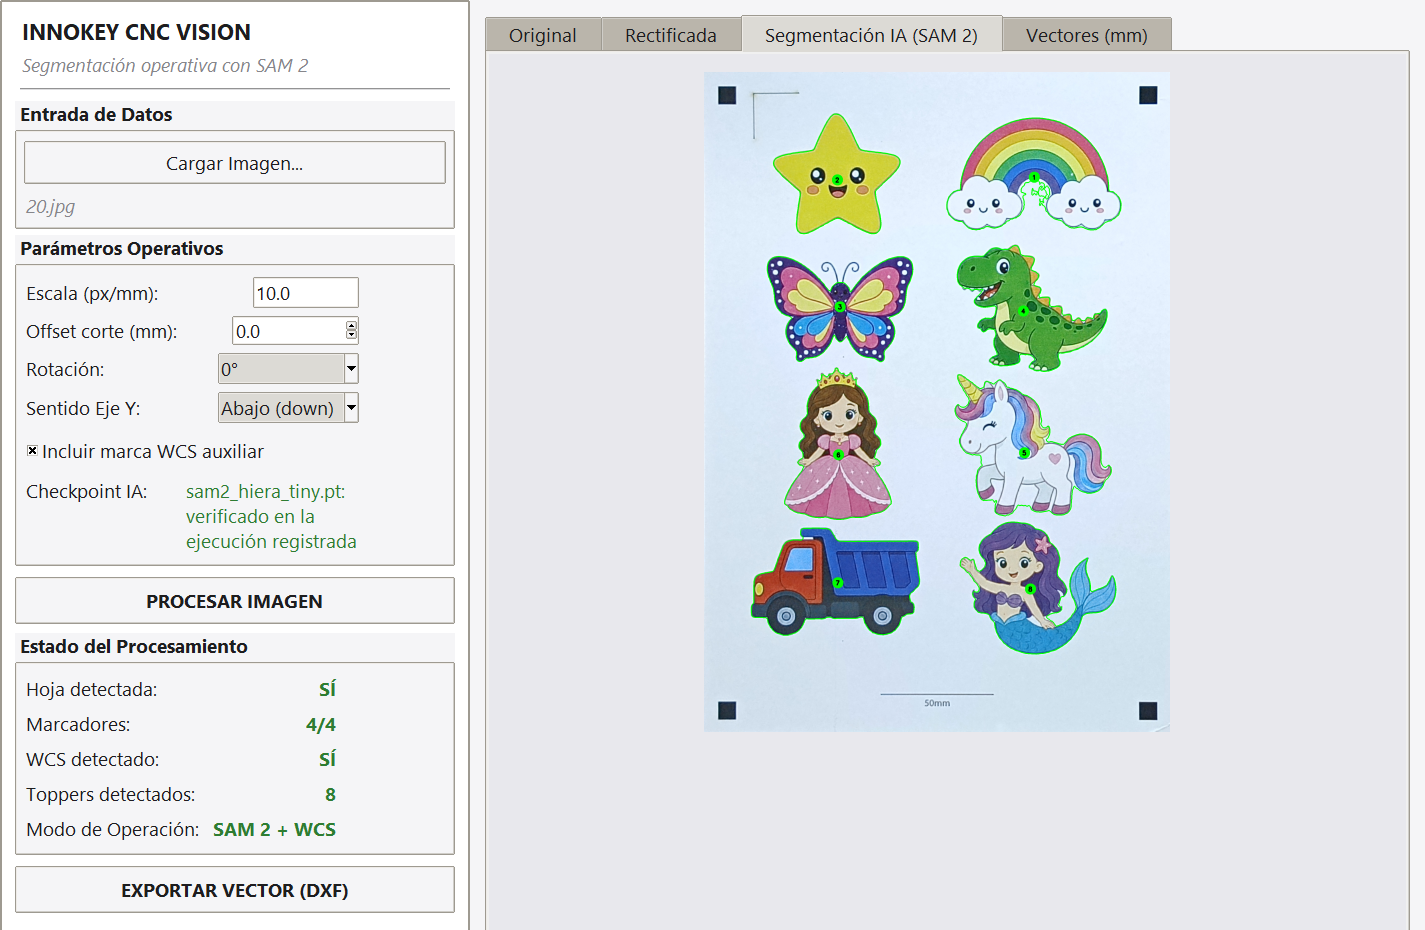
\includegraphics[width=0.90\linewidth]{figuras/interfaz_final/gui_final_03_sam2_document.png}
\captionof{figure}[Vista completa de la interfaz final.]{Vista completa de la interfaz tras procesar la captura 20 con SAM 2 y WCS.}
\label{fig:gui_sam2}
\end{landscape}

Para mantener legibles los controles y las pestañas, la ventana completa se presenta en formato apaisado en la Figura~\ref{fig:gui_sam2}. El detalle de la Figura~\ref{fig:gui_sam2_detalle} amplía los dos elementos que intervienen directamente en la decisión de exportar: el diagnóstico de la ejecución y la segmentación revisada por el usuario.

\figuraopcional{gui_sam2_legible}{0.92\textwidth}{Detalle ampliado del estado operativo y de la salida de SAM 2 en la captura 20.}{fig:gui_sam2_detalle}

La inspección no termina en la máscara. La pestaña vectorial representa en milímetros las ocho trayectorias exteriores y la referencia WCS que viajarán al DXF. La Figura~\ref{fig:gui_vectores} documenta esta segunda vista de la aplicación con una ampliación suficiente para revisar ejes, identificadores y capas.

\figuraopcional{gui_vectores_legible}{0.90\textwidth}{Previsualización vectorial de las ocho trayectorias exteriores y de la referencia WCS antes de utilizar el DXF en el flujo CAM.}{fig:gui_vectores}

\section{Verificación de la integración}

La integración se evaluó mediante 23 pruebas automatizadas y varias ejecuciones de extremo a extremo. Una parte del conjunto comprueba la configuración y los estados de la aplicación, incluidos el bloqueo de escala y las condiciones que habilitan la exportación. Otra recorre la geometría, desde la detección WCS en las trece capturas y el caso ambiguo con dos marcas en L hasta la selección del contorno exterior, los huecos opcionales, el offset y la reapertura del DXF. El contrato de inteligencia artificial se verifica aparte: el extractor debe recibir la máscara producida por SAM 2 y la ruta neuronal debe detenerse si falta el checkpoint, sin recurrir silenciosamente a la visión clásica.

En la captura 20, la herramienta detectó un WCS válido, generó ocho cajas, obtuvo ocho componentes con SAM 2 y extrajo ocho siluetas exteriores. Otra prueba controlada confirmó que el modo operativo descarta una perforación interna, aunque la función opcional puede conservarla cuando se solicita expresamente. El conjunto demuestra la continuidad del software y la coherencia estructural y geométrica interna del archivo. El comportamiento de esas trayectorias sobre el material deberá medirse en una campaña de corte.

\chapter{Resultados}
\label{cap:resultados}

Con las decisiones de datos, modelo, umbral y prompt ya cerradas, el capítulo comienza por la selección de los dos métodos de inteligencia artificial y continúa con la comparación de las tres rutas en los dominios sintético y real. También se presentan el coste temporal, el registro WCS y la integración hasta la exportación en formato DXF.

\section{Control de calidad del conjunto sintético}

La puerta de calidad aprobó las 48 hojas del conjunto \texttt{asset\_identity\_v2} sin registrar fallos críticos. El reparto quedó fijado en 24 hojas de entrenamiento, 12 de validación y 12 de prueba. Las 32 identidades de activo fueron únicas y no se encontraron coincidencias entre particiones en sus identificadores, nombres de archivo, hashes de origen, imágenes ni máscaras.

La auditoría también confirmó que todas las rutas existen, que las imágenes conservan las dimensiones de 2100 por 2970 píxeles y que las máscaras binarias y de instancia son válidas. Cada partición contiene las cuatro familias semánticas, las seis condiciones de captura y las dos distribuciones previstas.

Las doce hojas de validación reúnen siempre las mismas ocho identidades de ese subconjunto bajo dos distribuciones y seis condiciones. La prueba aplica el mismo esquema a otras ocho identidades. Este diseño permite comparar de forma controlada la respuesta ante las dos distribuciones y las seis condiciones, aunque las doce hojas no representan grupos independientes de productos.

\section{Optimización de Random Forest}

\subsection{Búsqueda y selección}

En la validación cruzada agrupada, C03 obtuvo el mayor Jaccard medio sobre píxeles, con $0{,}9737$. C07 quedó segundo con $0{,}9723$. El orden entre ambos cambió al reconstruir las hojas completas. C07, con umbral 0,55, alcanzó el mejor IoU de validación y mantuvo ocho componentes en todas las láminas.

\begin{table}[htbp]
\centering
\small
\caption{Segunda etapa de selección de Random Forest sobre doce hojas de validación.}
\label{tab:seleccion_rf}
\begin{tabularx}{\textwidth}{p{2.7cm}ccccY}
\toprule
\textbf{Candidato} & \textbf{Umbral} & \textbf{IoU} & \textbf{Dice} & \textbf{Error comp.} & \textbf{Procedencia} \\
\midrule
C07 & 0,55 & \textbf{0,9918} & \textbf{0,9959} & 0,00 & Segundo en validación cruzada \\
Control C00 & 0,60 & 0,9914 & 0,9956 & 0,00 & Configuración de referencia \\
C03 & 0,55 & 0,9913 & 0,9956 & 0,00 & Primero en validación cruzada \\
\bottomrule
\end{tabularx}
\end{table}

La Tabla~\ref{tab:seleccion_rf} muestra por qué la evaluación necesitó dos etapas: una diferencia pequeña sobre píxeles muestreados no basta para anticipar el comportamiento de una hoja completa. El modelo finalmente bloqueado usa 240 árboles, profundidad máxima 20, dos muestras mínimas para dividir, un mínimo de dos muestras por hoja terminal, 50 por ciento de las variables en cada división y ponderación balanceada, con un umbral de 0,55. La Figura~\ref{fig:rf_validacion_completa} recoge el resultado por lámina de los tres finalistas.

\begin{figure}[htbp]
\centering
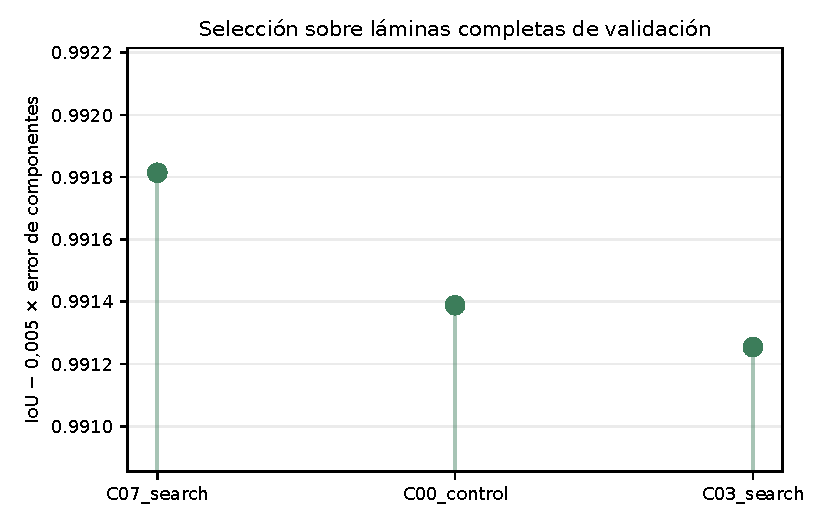
\includegraphics[width=0.93\textwidth]{../resultados/figuras/rf_idv2_full_sheet_validation.pdf}
\caption{IoU de los candidatos finalistas sobre las doce hojas completas de validación. La línea de selección combina solapamiento y error de componentes.}
\label{fig:rf_validacion_completa}
\end{figure}

\subsection{Ablación de características}

La ablación se realizó como diagnóstico sobre 24\,000 píxeles de validación y no intervino en la elección del modelo. Las nueve variables de color alcanzaron un Jaccard de $0{,}9523$. Añadir gradientes elevó el valor a $0{,}9636$, y el conjunto completo de 19 variables llegó a $0{,}9810$. Incorporar las coordenadas absolutas produjo $0{,}9800$. La Figura~\ref{fig:rf_ablacion} reúne esta comparación.

\begin{figure}[htbp]
\centering
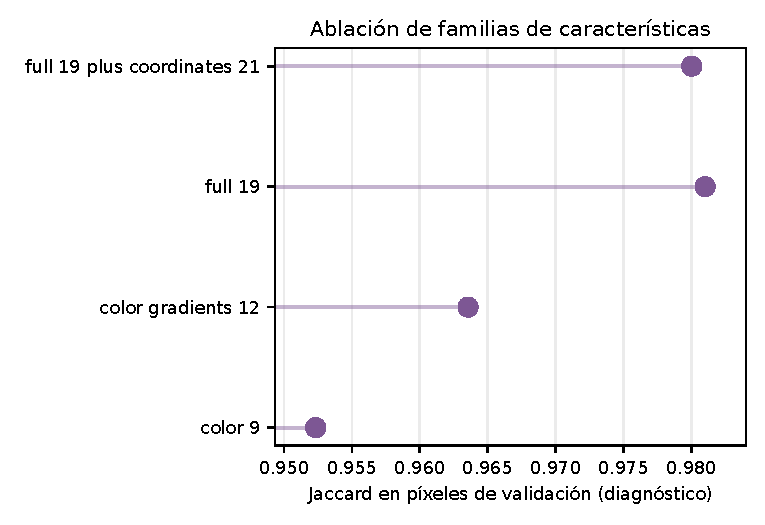
\includegraphics[width=0.86\textwidth]{../resultados/figuras/rf_idv2_feature_ablation.pdf}
\caption{Ablación diagnóstica de las variables de Random Forest sobre validación. El conjunto de 19 variables obtiene el mayor Jaccard en esta corrida, con una diferencia de 0,0010 respecto de la variante que añade coordenadas.}
\label{fig:rf_ablacion}
\end{figure}

La representación de 19 variables ya estaba bloqueada y no se modificó. El diagnóstico fue coherente con no añadir coordenadas: al incorporarlas, el Jaccard pasó de 0,9810 a 0,9800. El ensayo no permite atribuir la diferencia a un tipo concreto de borde, sombra o desenfoque ni establecer un efecto general de las coordenadas.

\section{Selección del margen de SAM 2}

Con cajas obtenidas por el mismo localizador de la aplicación, los cuatro márgenes conservaron ocho componentes. La Tabla~\ref{tab:seleccion_sam} reúne las métricas y la Figura~\ref{fig:sam_margen} representa la media junto con su intervalo de confianza. El 5 por ciento obtuvo el mayor IoU, aunque aventajó al 3 y al 10 por ciento en menos de cuatro diezmilésimas.

\begin{table}[htbp]
\centering
\small
\caption{Selección del margen de caja de SAM 2 sobre doce hojas de validación.}
\label{tab:seleccion_sam}
\begin{tabularx}{0.88\textwidth}{Ycccc}
\toprule
\textbf{Margen} & \textbf{IoU} & \textbf{Dice} & \textbf{Boundary F1} & \textbf{Error comp.} \\
\midrule
5 por ciento & \textbf{0,9232} & \textbf{0,9600} & 0,7663 & 0,00 \\
3 por ciento & 0,9228 & 0,9599 & \textbf{0,7685} & 0,00 \\
10 por ciento & 0,9228 & 0,9599 & 0,7579 & 0,00 \\
0 por ciento & 0,9214 & 0,9591 & 0,7679 & 0,00 \\
\bottomrule
\end{tabularx}
\end{table}

\begin{figure}[htbp]
\centering
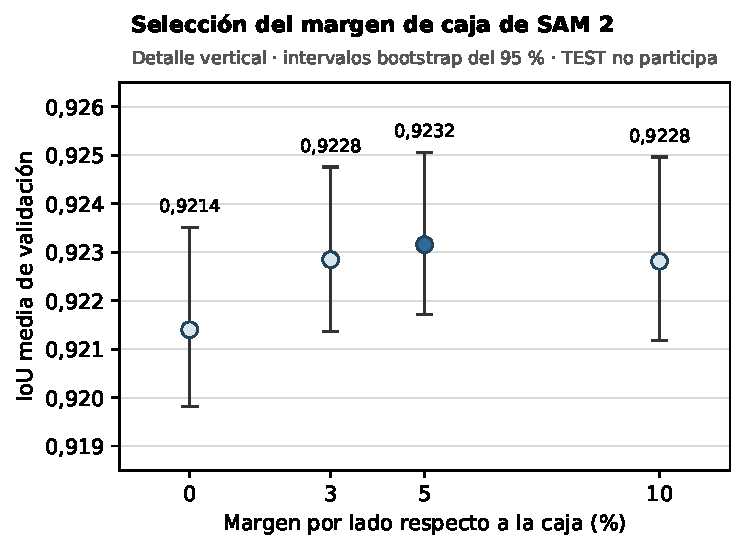
\includegraphics[width=0.82\textwidth]{../resultados/figuras_protocolo_v8/sam2_margin_selection_idv2.pdf}
\caption{Detalle de la IoU media para los cuatro márgenes evaluados. El eje vertical está restringido al intervalo 0,9185--0,9265 para hacer visibles diferencias de hasta 0,0018. Las barras de error son intervalos percentiles \textit{bootstrap} del 95 por ciento y se solapan ampliamente.}
\label{fig:sam_margen}
\end{figure}

El margen del 5 por ciento quedó bloqueado antes de abrir la prueba. Con ese valor, las cajas operativas y las ideales produjeron resultados casi idénticos: IoU de $0{,}92308$ y $0{,}92318$ en prueba, y concordancias de $0{,}95364$ y $0{,}95372$ en real. En las imágenes estudiadas, esta proximidad indica que la localización de las cajas no domina el error final.

\section{Comparación en prueba sintética}

Las doce hojas bloqueadas dejaron una diferencia clara entre el solapamiento de región y la fidelidad del borde. Random Forest encabezó IoU, Dice y Boundary F1, mientras que SAM 2 superó a la línea clásica en las dos métricas de región y la línea clásica conservó mayor coincidencia de contorno. La Tabla~\ref{tab:resultados_sinteticos} reúne los valores y la Figura~\ref{fig:comparacion_idv2} permite ver cómo se distribuyen entre láminas.

\begin{table}[htbp]
\centering
\small
\caption{Resultados finales sobre doce hojas sintéticas con identidades no vistas.}
\label{tab:resultados_sinteticos}
\begin{tabularx}{\textwidth}{Ycccc}
\toprule
\textbf{Método} & \textbf{IoU} & \textbf{Dice} & \textbf{Boundary F1} & \textbf{Error comp.} \\
\midrule
Visión clásica & $0{,}9098 \pm 0{,}0037$ & 0,9528 & 0,8039 & 0,00 \\
Random Forest & $\mathbf{0{,}9879 \pm 0{,}0089}$ & \textbf{0,9939} & \textbf{0,9412} & 0,00 \\
SAM 2 Hiera Tiny & $0{,}9231 \pm 0{,}0072$ & 0,9600 & 0,7376 & 0,00 \\
\bottomrule
\end{tabularx}
\end{table}

\begin{figure}[htbp]
\centering
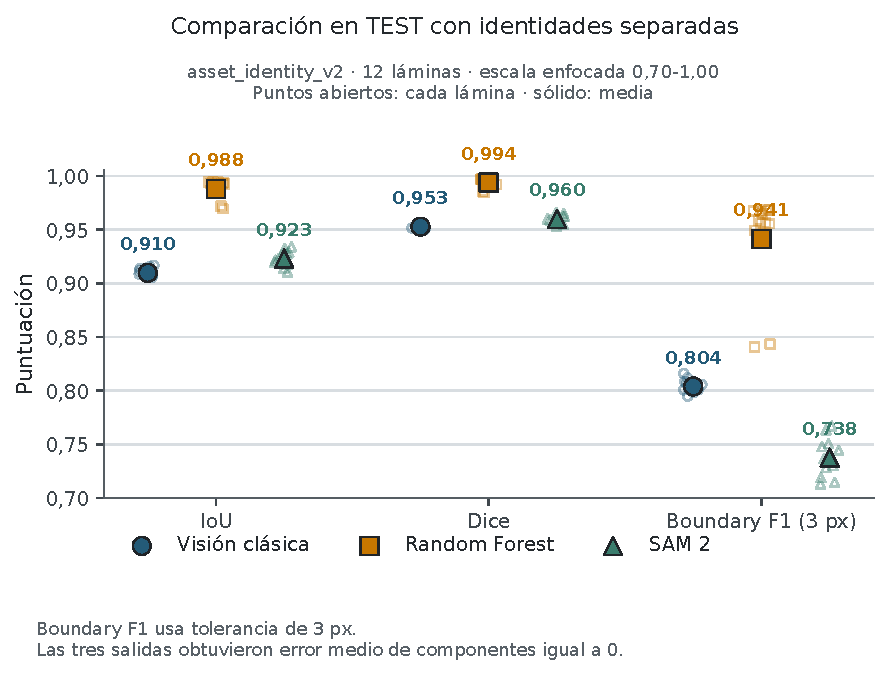
\includegraphics[width=0.96\textwidth]{../resultados/figuras/comparison_test_idv2_final.pdf}
\caption{Comparación de IoU, Dice y F1 de contorno en la prueba sintética con identidades separadas. Los marcadores abiertos corresponden a cada lámina y los sólidos muestran la media.}
\label{fig:comparacion_idv2}
\end{figure}

El desenfoque combinado con ruido de la condición C5 expuso la mayor sensibilidad de Random Forest: su IoU medio descendió a $0{,}9707$, cuando en C1, C2, C3 y C4 superaba $0{,}9917$, frente a $0{,}9839$ bajo la deformación ondulatoria C6. Esa pérdida afectó al solapamiento, pero no al recuento de objetos, pues las doce hojas conservaron el número correcto de componentes.

\section{Concordancia en las capturas reales}

Ningún parámetro se modificó al abrir la evaluación real. Según la Tabla~\ref{tab:resultados_reales}, la visión clásica presentó la mayor concordancia con la referencia canónica asistida. SAM 2 quedó $0{,}0251$ puntos por debajo y mantuvo las ocho instancias en las trece capturas. Random Forest descendió a $0{,}2881$ y produjo una sola región grande en todos los casos.

\begin{table}[htbp]
\centering
\small
\caption{Concordancia con la referencia asistida en trece vistas de una hoja real.}
\label{tab:resultados_reales}
\begin{tabularx}{\textwidth}{Ycccc}
\toprule
\textbf{Método} & \textbf{IoU} & \textbf{Dice} & \textbf{Boundary F1} & \textbf{Error comp.} \\
\midrule
Visión clásica & $\mathbf{0{,}9787 \pm 0{,}0159}$ & \textbf{0,9892} & \textbf{0,9069} & 0,00 \\
Random Forest & $0{,}2881 \pm 0{,}0037$ & 0,4473 & 0,2366 & 7,00 \\
SAM 2 Hiera Tiny & $0{,}9536 \pm 0{,}0083$ & 0,9763 & 0,7200 & 0,00 \\
\bottomrule
\end{tabularx}
\end{table}

Los intervalos percentiles \textit{bootstrap} del 95 por ciento para la media de IoU fueron $[0{,}9696,\,0{,}9863]$ para la línea clásica y $[0{,}9492,\,0{,}9577]$ para SAM 2. Describen la variación observada al remuestrear las trece capturas de una misma hoja y no sustentan una inferencia sobre productos independientes.

La región dominante generada por Random Forest se aprecia en la Figura~\ref{fig:rf_real}. El contraste descriptivo entre los dominios sintético y real se resume en la Figura~\ref{fig:brecha_dominios}, con la cautela de que sus referencias no son equivalentes.

\begin{figure}[htbp]
\centering
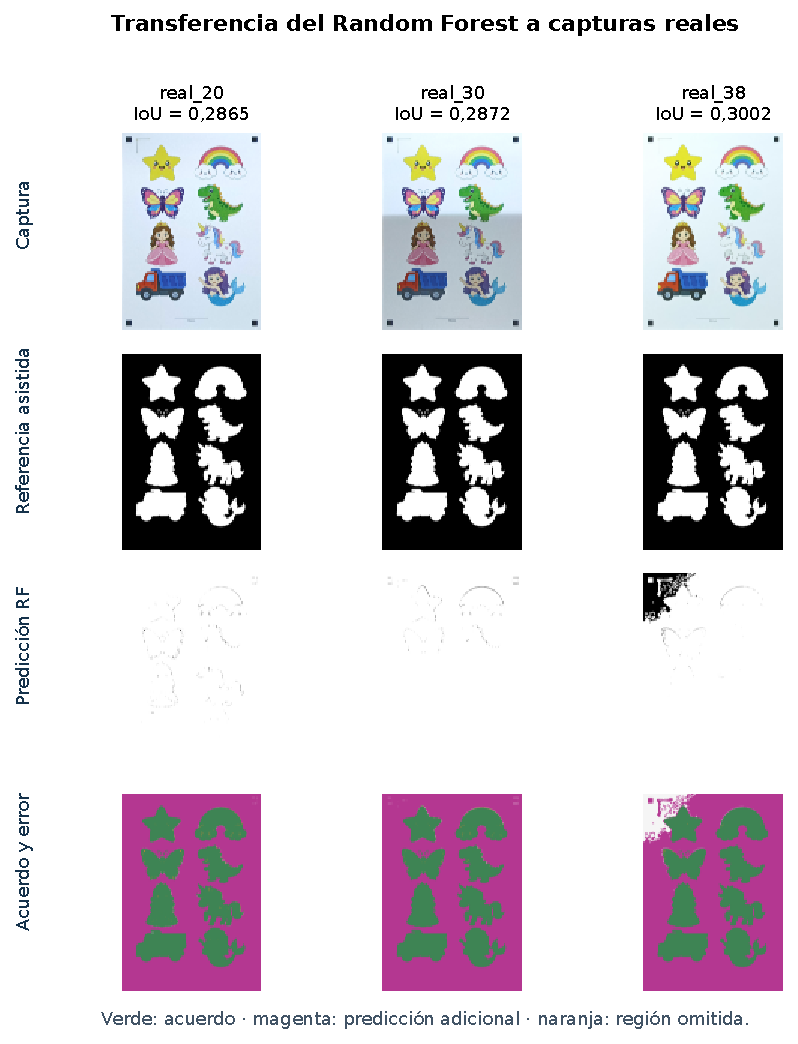
\includegraphics[width=0.94\textwidth]{../resultados/figuras/rf_idv2_real_agreement_examples.pdf}
\caption{Transferencia del Random Forest bloqueado a capturas reales. La predicción se extiende sobre una gran región de papel y no recupera las ocho siluetas.}
\label{fig:rf_real}
\end{figure}

\begin{figure}[htbp]
\centering
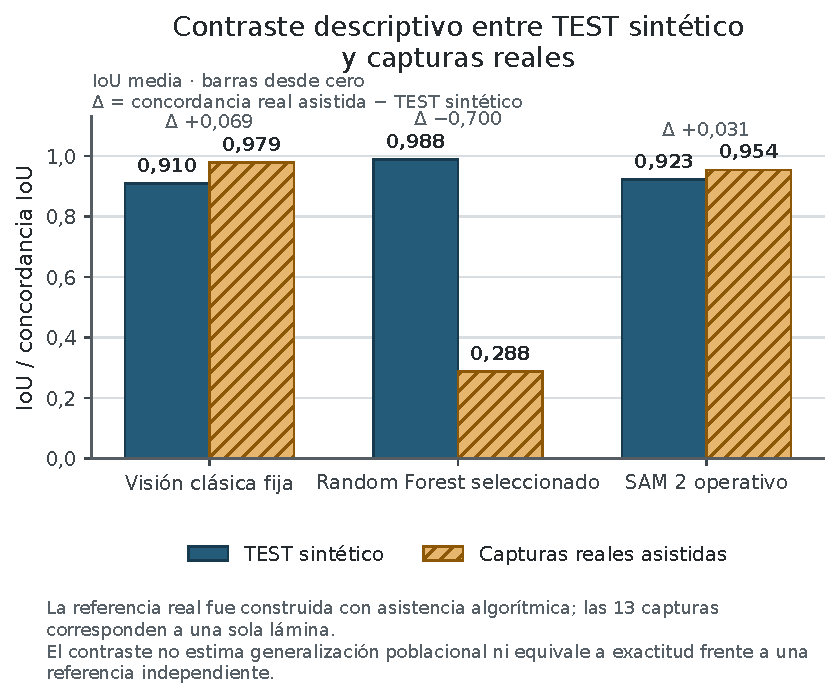
\includegraphics[width=0.94\textwidth]{../resultados/figuras/synthetic_real_gap_final.pdf}
\caption{Contraste descriptivo del IoU en la prueba sintética y de la concordancia IoU en las capturas reales. Las referencias no son equivalentes, por lo que la distancia entre barras documenta el cambio observado, pero no estima por sí sola transferencia ni generalización.}
\label{fig:brecha_dominios}
\end{figure}

\section{Coste temporal}

El banco temporal utilizó cuatro capturas rectificadas y precargadas, con un calentamiento y cinco repeticiones por imagen para cada método. Los tiempos de segmentación, medidos con el alcance homogéneo definido en la metodología, se presentan en la Tabla~\ref{tab:tiempos_segmentacion}.

\begin{table}[htbp]
\centering
\small
\caption{Tiempo de segmentación sobre CPU con imágenes precargadas, veinte mediciones por método.}
\label{tab:tiempos_segmentacion}
\begin{tabularx}{0.88\textwidth}{Yccc}
\toprule
\textbf{Método} & \textbf{Media (s)} & \textbf{Mediana (s)} & \textbf{Desv. (s)} \\
\midrule
Visión clásica & 0,1367 & 0,1330 & 0,0198 \\
Random Forest & 12,7163 & 12,1190 & 1,6652 \\
SAM 2 operativo & 2,1736 & 2,1430 & 0,2161 \\
\bottomrule
\end{tabularx}
\end{table}

Para SAM 2 se cronometró la ruta completa, desde el localizador hasta el postprocesamiento, incluido el codificador de imagen y no solo la decodificación de las cajas. Su media en CPU fue de $2{,}1736$ segundos. Esto equivale a 15,9 veces el tiempo de la línea clásica, mientras Random Forest necesitó 5,9 veces el tiempo de SAM 2. En este último método, los $12{,}7163$ segundos comprenden el cálculo de las 19 variables para más de seis millones de píxeles, la predicción de probabilidades y el postprocesamiento. Como las etapas no se cronometraron por separado, el total no puede atribuirse a una sola de ellas.

\section{Registro WCS y estabilidad entre capturas}

El detector encontró cuatro marcadores en las trece fotografías. Clasificó como válidas las diez que contienen la marca WCS y rechazó las capturas 13, 15 y 17. No hubo falsos positivos ni estados ambiguos en el conjunto real. La Tabla~\ref{tab:wcs_resultados} resume la clasificación y la dispersión observada.

\begin{table}[htbp]
\centering
\small
\caption{Resultado del registro geométrico sobre las capturas reales.}
\label{tab:wcs_resultados}
\begin{tabularx}{0.88\textwidth}{Yc}
\toprule
\textbf{Indicador} & \textbf{Resultado} \\
\midrule
Marcadores detectados & 13 de 13 capturas \\
Clasificación WCS & 10 positivas y 3 negativas, todas correctas \\
Desviación radial media del origen & 0,195 mm \\
Desviación radial máxima del origen & 0,390 mm \\
Desv. estándar del ángulo X & 0,085 grados \\
\bottomrule
\end{tabularx}
\end{table}

\begin{figure}[htbp]
\centering
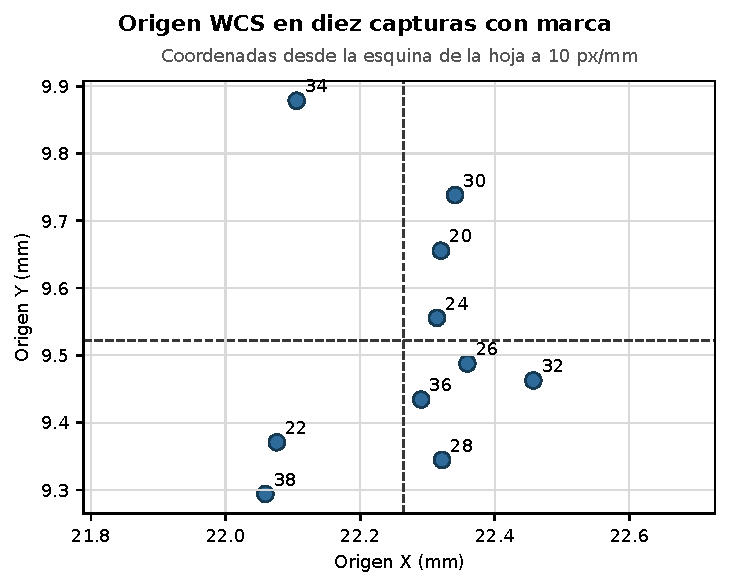
\includegraphics[width=0.80\textwidth]{../resultados/figuras_protocolo_v8/wcs_origin_repeatability_v8.pdf}
\caption{Dispersión del origen WCS recuperado en diez adquisiciones de la misma hoja. El centro representa la media observada, no una referencia metrológica independiente.}
\label{fig:wcs_repetibilidad}
\end{figure}

La Figura~\ref{fig:wcs_repetibilidad} representa la posición del origen recuperado en las diez capturas positivas respecto de su propia media. La estabilidad de máscaras se calculó entre los 45 pares posibles de esas capturas. La línea clásica obtuvo un IoU medio entre pares de $0{,}9644$ y SAM 2 de $0{,}9631$. Random Forest alcanzó $0{,}9883$, pero ninguna captura mantuvo ocho componentes. Esta última cifra describe una equivocación estable y no un mejor contorno.

\section{Integración y validación estructural del DXF}

Los cuatro marcadores se localizaron en las trece capturas y SAM 2 produjo ocho siluetas exteriores en la ruta operativa. El WCS se reconoció como válido en diez capturas y como ausente en tres, tal como correspondía. La aplicación exportó y reabrió los diez DXF autorizados, mientras que en los tres casos sin WCS bloqueó la salida. Así se evitó crear archivos sin una referencia geométrica aceptada. Cada DXF válido contenía ocho trayectorias de corte y no convirtió los vacíos internos de la máscara en perforaciones. Al reabrirlos se comprobaron las capas, el cierre de las polilíneas, la finitud de las coordenadas, el área no nula y unos límites plausibles. El alcance de estas comprobaciones es estructural: no equivale a una validación metrológica ni a una prueba de corte físico.

Las 23 pruebas automatizadas terminaron sin fallos y cubrieron la configuración, la escala, los estados de exportación, la ausencia y la ambigüedad del WCS, las siluetas exteriores, el modo opcional de huecos, el offset y la lectura de retorno del DXF. Con ello se verificó la continuidad entre módulos, aunque no el error entre una trayectoria calculada y un corte físico.

\chapter{Discusión}
\label{cap:discusion}

Los tres métodos no cubren el mismo alcance dentro del sistema, de modo que una sola métrica no basta para ordenarlos. La comparación cambia con el grado de control del entorno, el dominio de las imágenes y la forma de construir la referencia. Esas diferencias también condicionan qué método resulta viable dentro de la herramienta.

\section{Respuesta a las preguntas de evaluación}

La primera pregunta se responde al seguir la cadena completa y no solo una máscara aislada. SAM 2 mantuvo ocho instancias en las doce hojas sintéticas de prueba y en las trece capturas reales. Cuando el WCS era válido, sus máscaras dieron lugar a ocho trayectorias exteriores. La evidencia confirma la continuidad estructural del flujo, aunque todavía no establece la precisión geométrica necesaria para producción ni la calidad física del corte.

Random Forest también respondió bien dentro del dominio sintético. Su IoU de $0{,}9879$ se obtuvo sobre identidades que no aparecen en entrenamiento y no puede atribuirse a una repetición directa de los activos. Sin embargo, el modelo no conservó ese comportamiento en real. La salida se redujo a una región dominante y perdió siete de las ocho componentes esperadas.

El cambio entre dominios, objeto de la segunda pregunta, requiere una lectura cautelosa. SAM 2 obtuvo $0{,}9231$ frente a la referencia sintética y una concordancia de $0{,}9536$ frente a la referencia canónica real. Que la cifra real sea mayor no implica un mejor desempeño, porque ambas referencias se construyeron de forma distinta. Esa diferencia podría ser compatible con una escena rectificada de fondo claro y con el aislamiento espacial aportado por las cajas, pero una sola hoja no permite confirmarlo. Random Forest pasó de $0{,}9879$ a $0{,}2881$, una brecha marcada en el montaje evaluado.

\section{Alcance de la optimización de Random Forest}

La búsqueda de hiperparámetros separó las identidades mediante grupos, de modo que una misma identidad no aportara píxeles a ambos lados de un pliegue. Después, la reconstrucción de hojas completas evitó decidir solo con el Jaccard de una muestra balanceada. C07 no encabezó la etapa interna, pero fue el mejor sobre las doce láminas.

Las variables de color por sí solas ya aportaban gran parte de la capacidad de separación dentro del generador. Los gradientes y el contexto local mejoraron el Jaccard, mientras que las coordenadas no aportaron ventaja. Esto reduce el riesgo de que el modelo memorice la plantilla, pero no elimina el problema fotométrico: las variables continúan ligadas a intensidades, estadísticas de vecindad y escalas definidas en el corpus sintético.

El fracaso en las capturas reales no invalida Random Forest para cualquier tarea de segmentación industrial. Sí muestra que este modelo, entrenado únicamente con las simulaciones del estudio, no se transfirió al montaje. Ajustarlo tras observar las trece capturas quizá habría elevado la cifra, a costa de convertir la evaluación externa en un nuevo conjunto de validación. Por eso se conservó el resultado bloqueado.

\section{SAM 2 como componente de inteligencia artificial}

Sin superar a la línea clásica en concordancia real, SAM 2 mantuvo estable el número de instancias y mostró una diferencia entre dominios mucho menor que Random Forest, aun sin haberse entrenado con las imágenes del proyecto. Este comportamiento es compatible con una representación preentrenada menos ligada al color exacto del generador. La comparación, sin embargo, no aísla ese efecto porque también cambian la arquitectura, los prompts y la supervisión.

La arquitectura sigue siendo híbrida porque SAM 2 recibe las cajas del localizador clásico. Para estimar cuánto dependía de ellas se compararon cajas ideales y operativas. Las diferencias de IoU fueron inferiores a una diezmilésima tanto en prueba como en real, lo que indica que las cajas disponibles bastaron en este banco. El error restante se relaciona principalmente con la máscara generada por SAM 2 y con su contorno.

El contorno sí requiere atención. Aunque SAM 2 superó a la línea clásica en IoU sintético, quedó por debajo en Boundary F1, y esa desventaja de borde se repitió en real. Parte de la diferencia procede de pequeñas irregularidades y vacíos internos. Por ese motivo, el programa no convierte automáticamente todos los niveles de la máscara en rutas. Exportar solo la envolvente exterior evita que ojos o brillos impresos terminen como perforaciones.

La elección de SAM 2 para la interfaz respondió al objetivo de construir una herramienta basada en inteligencia artificial y a su comportamiento operativo, no a que fuera el mejor en todas las métricas. Es el modelo que genera la máscara vectorizada, conserva las ocho instancias y comunica el fallo si no puede inicializarse. La línea clásica se mantiene como referencia experimental, apoyo geométrico y posible alternativa práctica para la empresa fuera del alcance académico.

\section{Interpretación de la ventaja clásica}

Que la visión clásica alcanzara una concordancia real de $0{,}9787$, frente a $0{,}9536$ de SAM 2, resulta plausible en un entorno de fondo claro, hoja conocida, rectificación y colores impresos para el que se diseñaron sus reglas. El experimento no separa el efecto de cada condición. Sí muestra que, en la escena estudiada, una solución específica puede coincidir más con la referencia que un modelo general.

La comparación, sin embargo, presenta una asimetría metodológica. La referencia canónica se construyó con cajas del localizador clásico, GrabCut, Canny y morfología. No copia la máscara clásica, pero comparte parte del procedimiento y puede favorecer un tipo de borde semejante. El $0{,}9787$ describe, por ello, una concordancia alta con la preanotación disponible y no una exactitud física independiente.

Una anotación manual independiente podría modificar las diferencias observadas, en especial en antenas, patas, cabello y en la abertura del arcoíris. Aportaría además un criterio externo para decidir si un borde más suave de SAM 2 resulta preferible para el láser aunque su Boundary F1 sea menor.

\section{Registro geométrico y alcance estructural del DXF}

El sistema clasificó correctamente el WCS en las trece capturas y respondió también ante un caso sintético ambiguo. La dispersión radial media de $0{,}195\,\text{mm}$ y la desviación estándar del ángulo del eje X de $0{,}085$ grados muestran repetibilidad entre adquisiciones. No miden exactitud absoluta porque no existe una referencia metrológica externa.

La lectura de retorno de diez DXF aporta una verificación más fuerte que comprobar únicamente que el archivo no esté vacío. Las polilíneas son cerradas, finitas y coherentes con el número de siluetas. Aun así, una geometría válida puede producir un corte desalineado si la cámara conserva distorsión radial, si la marca WCS se graba con error o si la máquina introduce holgura.

El offset permanece en cero por la misma razón. Su aplicación matemática funciona y no se omite cuando falta una dependencia, pero el valor apropiado depende del ancho real del haz, del material, de la potencia y de la velocidad. Elegirlo sin una campaña física daría una apariencia de precisión no respaldada.

\section{Coste computacional y uso en taller}

El tiempo de la línea clásica es el menor porque opera con transformaciones locales. Random Forest debe calcular 19 variables para más de seis millones de píxeles y después evaluar cientos de árboles. SAM 2 codifica la imagen una vez y decodifica ocho cajas. En CPU no ofrece respuesta instantánea. La media de $2{,}17$ segundos permitió completar el flujo del prototipo, aunque su aceptabilidad para producción no se evaluó con operarios ni mediante un requisito temporal externo.

La medición excluye la carga inicial del modelo y la lectura desde disco. En una sesión de trabajo, el checkpoint se carga una vez y el coste se amortiza. Una GPU reduciría la espera, aunque no corregiría por sí sola los errores de borde. Para producción importan tanto el tiempo como la posibilidad de inspeccionar la máscara y bloquear una exportación dudosa.

\section{Amenazas a la validez}

\subsection{Validez interna}

La separación por identidad y el bloqueo de prueba reducen la contaminación. Persisten, sin embargo, decisiones incorporadas al generador, como el fondo, el tamaño de los activos y las seis degradaciones. Los umbrales clásicos proceden del desarrollo previo y la gráfica HSV sirve para describirlos, no para convertirlos en un método optimizado bajo el mismo presupuesto que Random Forest.

\subsection{Validez de constructo}

IoU, Dice y Boundary F1 miden propiedades de una máscara. No miden directamente acabado, ancho de haz ni aceptación del cliente. El F1 de contorno usa una tolerancia de tres píxeles y una coincidencia por dilatación, no el emparejamiento uno a uno del protocolo BSDS. El error de componentes se acerca más a la vectorización, pero tampoco garantiza que todos los detalles geométricos sean fabricables.

\subsection{Validez externa}

Las ocho identidades de prueba sintética son nuevas para los modelos, aunque se repiten en doce combinaciones. El dominio real solo contiene una hoja, un teléfono, una máquina y un conjunto de ocho diseños. No se evaluaron otros materiales, cámaras, tamaños ni talleres. En consecuencia, la evidencia respalda el prototipo y su montaje, no una tasa de acierto poblacional.

\subsection{Validez de la referencia}

La preanotación real es canónica y asistida. Las trece copias de referencia son idénticas porque representan el mismo plano físico. Esto es coherente para estudiar variación de captura, pero impide tratar cada archivo como una etiqueta independiente. La inspección visual disponible tampoco equivale a un acuerdo entre anotadores.

\section{Síntesis}

El balance es desigual y, precisamente por ello, informativo. Random Forest dominó dentro del generador y perdió siete componentes al transferirse, mientras la línea clásica fue la que más coincidió con la referencia real asistida. SAM 2 quedó entre ambas en las métricas, pero fue el único de los dos métodos de inteligencia artificial que conservó las ocho instancias en los dos dominios y completó la ruta operativa de la interfaz. El aporte académico consiste en delimitar ese comportamiento dentro del montaje estudiado, integrarlo con comprobaciones explícitas y dejar identificadas las pruebas necesarias antes de usar la salida como orden de producción.

\chapter{Conclusiones y trabajo futuro}
\label{cap:conclusiones}

\section{Conclusiones}

La interfaz desarrollada reúne en una sola ruta el registro de la hoja impresa, la segmentación de sus ocho diseños con SAM 2 y la conversión de las siluetas exteriores en trayectorias DXF referidas al WCS del láser. El cambio de proceso que la sustenta es concreto: la hoja completa se adhiere primero al soporte y el corte se calcula sobre la posición real de la impresión.

La participación de la inteligencia artificial puede seguirse hasta la salida. SAM 2 produjo la máscara que recibió el extractor de contornos tanto en la interfaz como en la ejecución por lote. Sobre doce hojas sintéticas con identidades no vistas obtuvo un IoU de $0{,}9231$ y en las trece adquisiciones de una hoja real alcanzó una concordancia de $0{,}9536$, conservando las ocho instancias en todas ellas.

El orden de los métodos cambió con el dominio: la línea clásica alcanzó la mayor concordancia real, $0{,}9787$, en un montaje acotado de fondo claro, marcadores conocidos y reglas adaptadas al proceso. Random Forest, en cambio, obtuvo el mejor IoU sintético, $0{,}9879$, después de la búsqueda agrupada y de la selección sobre hojas completas, pero descendió a $0{,}2881$ en real y no conservó los ocho componentes en ninguna captura, con una diferencia descriptiva entre ambos dominios de $0{,}6999$. Estas cifras no invalidan el uso operativo de SAM 2 ni permiten una clasificación poblacional, porque el conjunto sintético dispone de etiquetas exactas y el real utiliza una referencia asistida. Sí documentan que una técnica específica puede aventajar a un modelo general en una escena controlada y que un aprendizaje eficaz en sintético puede no transferirse al taller.

En la parte geométrica, el WCS se clasificó correctamente en las trece capturas. La desviación radial media del origen fue de $0{,}195\,\text{mm}$ y la desviación estándar del ángulo del eje X, de $0{,}085$ grados. Los diez DXF autorizados se reabrieron con ocho polilíneas exteriores válidas, mientras las tres imágenes sin WCS utilizable quedaron bloqueadas. Se demostró así consistencia computacional, no todavía el error físico de corte.

La revisión de las máscaras llevó además a una decisión de seguridad. Sus vacíos internos correspondían a ojos, brillos o pequeñas imperfecciones y no a perforaciones deseadas. Por eso, la aplicación exporta por defecto únicamente la silueta exterior. El soporte de huecos permanece como una opción explícita para otras piezas, fuera del flujo validado aquí.

\section{Cumplimiento de los objetivos}

El objetivo general se considera cumplido dentro del alcance definido para el software y la evaluación experimental. La herramienta usa SAM 2 como segmentador operativo, conserva la referencia física y entrega un DXF estructuralmente validado cuando existe un WCS inequívoco. La Tabla~\ref{tab:cumplimiento_objetivos} relaciona cada objetivo específico con su evidencia.

\begin{table}[htbp]
\centering
\small
\caption{Trazabilidad de los objetivos específicos y su evidencia.}
\label{tab:cumplimiento_objetivos}
\begin{tabularx}{\textwidth}{p{1.7cm}Y}
\toprule
\textbf{Objetivo} & \textbf{Evidencia principal} \\
\midrule
OE1 & Montaje con teléfono, soporte removible, hoja A4 y trece capturas bajo cambios de sombra y posición. \\
OE2 & Cuatro marcadores detectados en trece capturas, rectificación A4 y clasificación WCS correcta en diez casos positivos y tres negativos. \\
OE3 & 32 activos y 48 hojas con separación de identidades 16/8/8, auditoría de hashes y cero solapamientos. \\
OE4 & Diez configuraciones, cuatro pliegues agrupados, selección sobre doce hojas y bloqueo de C07 con umbral 0,55. \\
OE5 & Selección del margen del 5 por ciento en validación, prueba sintética, concordancia real e integración de SAM 2 en la interfaz. \\
OE6 & Extracción de ocho siluetas exteriores, transformación a milímetros y exportación DXF condicionada al WCS. \\
OE7 & Comparación mediante IoU, Dice, F1 de contorno, componentes y tiempo, con límites de la referencia real declarados. \\
\bottomrule
\end{tabularx}
\end{table}

Queda fuera de lo demostrado cualquier reducción de reprocesos: para sostenerla harían falta piezas cortadas, mediciones físicas y una comparación con el proceso manual. Tampoco puede afirmarse generalización a otros productos, ya que las capturas reales proceden de una sola hoja.

\section{Aportes}

Una aportación central es la arquitectura híbrida: la visión clásica resuelve el registro y la localización aproximada, mientras SAM 2 genera la máscara operativa. La interfaz hace visible esta separación y las pruebas impiden una sustitución silenciosa.

El protocolo de evaluación parte de la unidad de datos. Las identidades gráficas son disjuntas entre entrenamiento, validación y prueba. Para Random Forest quedaron documentadas las 19 variables, la búsqueda de hiperparámetros, la validación agrupada, la selección por hoja y el bloqueo verificable.

La comparación distingue el solapamiento, el borde, los componentes y la transferencia. Los resultados muestran tres comportamientos: la especialización sintética de Random Forest, la eficacia específica de la línea clásica y la estabilidad de SAM 2 en el número de componentes, con una brecha aparente menor entre las cifras de ambos dominios.

La cadena de salida añade una protección operativa. La escala tiene un único valor validado, la ausencia o ambigüedad del WCS bloquea la exportación y el DXF se escribe de forma atómica antes de reabrirse. Las 23 pruebas automatizadas documentan estos contratos.

\section{Trabajo futuro}

La evaluación en dominio real se apoya en una sola hoja, y esa restricción es la limitación experimental más importante. Una ampliación útil debería reunir varias hojas, diseños no observados, cámaras, materiales e iluminaciones, con máscaras anotadas manualmente y revisadas por más de una persona. Ese banco permitiría estimar la generalización, revisar la aparente ventaja clásica y estudiar un detector ligero, adaptadores o el ajuste fino de SAM 2 sin reutilizar la evaluación. Para Random Forest, el paso razonable consiste en incorporar ejemplos fotográficos y comprobar si las variables dejan de confundir el papel con el primer plano, no en ampliar la búsqueda de forma indiscriminada.

Pasar del software al material exigirá cortar MDF y acrílico, medir la distancia entre el borde impreso y el mecanizado, comprobar la escala en distintos puntos y estimar el ancho del haz. Esos ensayos permitirán fijar el offset y relacionar las métricas de imagen con la calidad que percibe el cliente. Si aparecen errores sistemáticos, una calibración intrínseca del teléfono podrá corregir la distorsión antes de la homografía, y una marca WCS de brazos más largos o varias referencias distribuidas podrán reducir la sensibilidad angular lejos del origen.

Acercar el prototipo al uso cotidiano requerirá un instalador, una comprobación guiada del checkpoint, aceleración por GPU, registro de lotes y automatización de la lectura y del procesamiento por lote. Una integración más directa con RDWorks solo debería abordarse después de validar físicamente la salida y conservar una revisión antes de enviar la orden de corte. Cualquier ampliación deberá mantener los bloqueos actuales y la inspección visual previa.


\appendix
\renewcommand{\appendixname}{ANEXO}
\chapter{Repositorio y reproducibilidad}
\label{ap:repositorio}

Este apéndice describe cómo reconstruir las evaluaciones y ejecutar la herramienta. El repositorio entregado conserva código, configuraciones, métricas y figuras. Los archivos de modelos de gran tamaño se verifican por nombre, tamaño y SHA-256. Las rutas que contienen datos o checkpoints pueden ajustarse en \texttt{software/config/default.yaml}.

\section{Estructura principal}

\begin{description}
    \item[\texttt{memoria/}] Fuentes \LaTeX, bibliografía y figuras de la memoria.
    \item[\texttt{software/}] Aplicación, interfaz gráfica, configuración y pruebas.
    \item[\texttt{datos/}] Manifiesto, particiones, anotaciones y capturas requeridas por los experimentos.
    \item[\texttt{experimentos/}] Scripts de calidad, Random Forest, SAM 2 y comparación.
    \item[\texttt{resultados/}] Métricas CSV/JSON, predicciones, modelos y evidencias de integración.
    \item[\texttt{documentacion/}] Protocolo experimental, trazabilidad y matriz de observaciones.
    \item[\texttt{output/pdf/}] Memoria final compilada.
\end{description}

\section{Preparación del entorno}

En Windows PowerShell, el entorno base puede prepararse con:

\begin{verbatim}
python -m venv .venv
.\.venv\Scripts\Activate.ps1
python -m pip install --upgrade pip
pip install -r requirements-core.txt
pip install -r requirements-ai.txt
\end{verbatim}

La instalación de SAM 2 puede depender de las versiones de Python y PyTorch disponibles. La evaluación final se ejecutó en CPU con Python 3.14.0, PyTorch 2.12.1+cpu, OpenCV 4.13.0 y scikit-learn 1.9.0. Estos datos también quedan almacenados en los resúmenes JSON.

\section{Modelos utilizados}

\begin{table}[htbp]
\centering
\scriptsize
\caption{Identificación de modelos y checkpoints.}
\label{tab:checksums_modelos}
\begin{tabularx}{\textwidth}{p{3.5cm}p{2.0cm}Y}
\toprule
\textbf{Archivo} & \textbf{Tamaño} & \textbf{SHA-256} \\
\midrule
\path{sam2_hiera_tiny.pt} & 155,906,050 B & \ttfamily\seqsplit{65B50056E05BCB13694174F51BB6DA89C894B57B75CCDF0BA6352C597C5D1125} \\
\path{random_forest_legacy_v1.joblib} & 60,111,985 B & \ttfamily\seqsplit{B6141FB7DB8320D9A33155F38BF0EFE1AC6FAE15195462548B1D50DDA5627836} \\
\path{random_forest_legacy_v2.joblib} & 233,889,745 B & \ttfamily\seqsplit{4B8D8ED8EE2D7E51C7F93AC50A8E9035AFE1D0BE58462A81E9DB18902E7C3911} \\
\bottomrule
\end{tabularx}
\end{table}

La fuente oficial del checkpoint SAM 2 es el repositorio de Meta. Deben respetarse su licencia y las condiciones del proyecto original. Los modelos Random Forest se generan con los scripts y datos de esta entrega. No es necesario conservarlos si se prefiere reconstruirlos.

\section{Comandos de reproducción}

Los comandos siguientes se ejecutan desde la raíz del repositorio:

\begin{verbatim}
python experimentos/construir_manifiesto.py

python experimentos/comparacion/crear_referencia_real_asistida.py

python experimentos/random_forest/optimize_rf_v7.py
python experimentos/random_forest/refine_rf_on_validation.py
python experimentos/random_forest/evaluate_rf_v1_control.py
python experimentos/random_forest/consolidate_rf_selection.py

python experimentos/sam2/evaluate_sam2_v7.py
python experimentos/sam2/evaluate_sam2_real_v7.py

python experimentos/comparacion/evaluate_classical_synthetic_v7.py
python experimentos/comparacion/evaluate_classical_rf_real_v7.py
python experimentos/comparacion/generar_figuras_v7.py

python -m unittest discover software/tests -v
\end{verbatim}

La búsqueda de Random Forest es la etapa de mayor duración. Los archivos finales que justifican la selección son:

\begin{itemize}
    \item \path{rf_hyperparameter_search.csv}.
    \item \path{rf_validation_model_threshold_summary.csv}.
    \item \path{rf_v1_control_selection.json}.
    \item \path{rf_consolidated_selection.json}.
\end{itemize}

En SAM 2, la estrategia se registra en \path{sam2_final_selection.json}.

\section{Ejecución de la herramienta}

La interfaz puede abrirse con:

\begin{verbatim}
python software/src/gui.py
\end{verbatim}

Para una demostración reproducible puede precargarse y procesarse una imagen:

\begin{verbatim}
python software/src/gui.py --image datos/reales/raw/20.jpg --process
\end{verbatim}

La interfaz no vuelve de forma silenciosa al método clásico. Si el checkpoint de SAM 2 no existe o no puede inicializarse, la operación falla con un mensaje. La exportación DXF permanece deshabilitada hasta detectar un WCS válido.

\section{Publicación}

El código fuente, la memoria compilada y los resultados reproducibles están disponibles en el siguiente repositorio público:

\begin{center}
\small\url{https://github.com/bryangr1993/tfm-vision-artificial-sam2}
\end{center}

La versión 6 se conservó fuera de su historial de edición. Los checkpoints y modelos pesados no forman parte del repositorio ordinario debido a su tamaño. Pueden distribuirse mediante una versión de GitHub o un almacenamiento externo, siempre acompañados por los checksums de la Tabla~\ref{tab:checksums_modelos}.


\begingroup
\small
\bibliographystyle{apacite}
\bibliography{bibliografia}
\endgroup

\end{document}
